The present thesis combines methods from the fields of integer linear programs (ILP), machine learning and statistical inference. This chapter aims to provide the reader with sufficient background information and notations to tackle the following chapters. In the first section we will give a presentation of ILPs and their formal definition as well as a brief overview of strategies for solving such problems, emphasizing the elements that could be subject to integration of ML techniques. Machine learning, being the central approach that we aim to study in relation to ILPs will be presented in the following section. We follow this presentation by defining Markov Random Fields and the general inference problem that will be required and refered to throughout the contribution work of this thesis.


\section{Integer Linear Programming}
\label{sec:co_intro}
\label{chap:chapter_1.1_integer_linear_programming}

This section introduces the integer linear programming framework used in the main contributions of this thesis. We focus mainly on binary integer linear programs (BILPs), in which decision variables take values in $\{0,1\}$ and feasibility is determined by a system of linear constraints. This setting is general enough to encode many classical combinatorial optimization problems, while also exposing the central difficulty studied in this thesis: predicting or constructing binary assignments whose variables are strongly coupled by feasibility constraints. We first define the ILP formalism, then briefly review classical solver components, and finally introduce the graph representations and benchmark problems used in later chapters.

\subsection{Combinatorial optimization and ILP formulations}

Combinatorial optimization (CO) concerns optimization problems whose feasible solutions are discrete objects, such as subsets, paths, matchings, or assignments. Many such problems can be formulated as integer linear programs, which makes ILPs a convenient common language for both classical optimization algorithms and learning-based methods. In this thesis, we focus on binary ILP formulations that explicitly expose variables and constraints, since this structure can be represented as a graph and used as input to neural and graphical-model methods.

\subsection{Problem definition}
The \emph{canonical form} of an ILP is given as
\begin{equation}
    \label{equ:ilp_canonical_form}
    (P) \Leftrightarrow \left\{
    \begin{aligned}
        \max \quad & c^\top x \\
        \text{s.t.} \quad & Ax \leq b, \\
        & x \in \mathcal{X}
    \end{aligned} \right. ,
    % \begin{array}{ll}
    %     \max & c^T x \\
    %     \text{s.t.}              & A x \leq b \\
    %                              & x \in \mathcal{X}
    % \end{array}
\end{equation}
where $x\in \mathcal{X} \subseteq \Z^n$ denotes the vector of decision variables, $c\in\R^n$ is the objective coefficient vector, and $A\in\R^{m\times n}$ and $b\in\R^m$ define the linear constraints. We write $A_j$ for the $j$-th row of $A$, so that the $j$-th constraint is $A_jx \leq b_j$. 

Binary integer linear programs (BILPs), which are the main focus of this thesis, are problems for which $\mathcal{X}=\{0,1\}^n$. An assignment $x$ is called \emph{feasible} if it satisfies both the domain restrictions and the linear constraints; the feasible set is therefore $\FEASIBLESET := \{x\in\mathcal{X} : Ax \leq b\}$.

A formulation is said to be \emph{compact} if the number of variables and constraints is polynomial in the size of the input~\cite{yannakakis_expressing_1988,carr_compact_2000}. This assumption is important for the methods developed in this thesis, since the variable-constraint graph must be represented explicitly. We therefore focus mainly on problems that admit compact BILP formulations. Compactness, however, does not imply that every constraint is small: a compact formulation may still contain constraints involving many variables. This distinction will become important later when we represent constraints through graphical-model structures.

\subsubsection{LP relaxations and solver-state quantities}
Given a BILP with feasible set $\mathcal{X}=\{0,1\}^n$, its linear programming relaxation is obtained by replacing the integrality constraints with continuous bounds:
\begin{equation}
(P_{\mathrm{LP}}) \Leftrightarrow \left\{
\begin{aligned}
\max \quad & c^\top x \\
\text{s.t.} \quad & Ax \leq b, \\
& 0 \leq x \leq 1 .
\end{aligned} \right. .
\end{equation}
The resulting LP provides a continuous approximation of the original integer problem. A point is LP-feasible if it satisfies the linear constraints and the relaxed bounds; it is integer-feasible if it also satisfies the original integrality restrictions. Thus, an LP-feasible solution may be fractional, meaning that some variables satisfy $0<x_i^{\mathrm{LP}}<1$.

LP relaxations provide both bounds for exact solvers and useful information for heuristics and learning models. For a constraint $A_jx\leq b_j$, the slack at an LP solution $x^{\mathrm{LP}}$ is
\begin{equation*}
s_j = b_j - A_jx^{\mathrm{LP}}.
\end{equation*}
A constraint is active, or tight, when $s_j=0$. LP solvers also return dual values associated with constraints, which can be interpreted as sensitivities of the LP objective to changes in the right-hand side, and reduced costs associated with variables, which indicate how variable movements would affect the LP objective around the current optimum.

When the relaxation is solved by the simplex method, the solution is represented by a basis. The corresponding basis status of a variable or constraint records whether it is basic or nonbasic, and, if nonbasic, which bound is active. These quantities are often exposed by MILP solvers and will later be used as optimization-aware features in the variable-constraint graph representation.


\subsection{Solving ILPs}

ILPs can be approached either with algorithms tailored to a specific combinatorial problem or with general-purpose optimization methods. Specialized algorithms can be highly efficient when they exploit additional structure, but they do not provide a uniform framework for arbitrary ILP formulations. In contrast, general-purpose ILP solvers operate directly on the algebraic formulation. This thesis largely follows the latter perspective: the methods developed later take a BILP formulation as input, while using its constraint structure to build graph-based learning and inference models. We therefore briefly review the main solver components that motivate learning-augmented ILP methods.

\subsubsection{Exact approaches}
The most straightforward but impractical approach is exhaustive enumeration of all candidate solutions. More sophisticated exact algorithms exploit structure to prune the search space.

\paragraph{Branch-and-Bound} The Branch-and-Bound (B\&B) method~\cite{land_automatic_1960,dakin_tree-search_1965} explores the solution space through a search tree. At each node, the problem is restricted by branching on a decision variable, yielding subproblems that can be pruned using bounds, infeasibility, or integrality. Figure~\ref{fig:branch_and_bound_tree} illustrates this search-tree structure.

Although B\&B is exact, its worst-case complexity remains exponential, and its practical performance depends heavily on choices such as variable selection, node selection, branching direction, and primal heuristics. These choices provide natural points of intervention for learning-augmented solvers, as reviewed in Chapter~\ref{chap:chapter_2_related_work}. Table~\ref{tab:branch_and_bound_strategies} summarizes these decision points, many of which have been targeted by learning-based methods. Classical examples include strong branching, pseudo-cost and reliability branching, feasibility-pump heuristics, RINS, and local branching~\cite{achterberg_branching_2005,benichou_experiments_1971,fischetti_feasibility_2005,danna_exploring_2005,fischetti_local_2003}.

% \begin{figure}[h!]
% \centering
% \begin{forest}
% for tree={
%     draw,
%     rounded corners,
%     align=center,
%     minimum width=2.2cm,
%     minimum height=1cm,
%     inner sep=2pt,
%     font=\small
% },
% good/.style={fill=green!20},
% bad/.style={fill=red!20},
% neutral/.style={fill=blue!10}
% [P$_0$\\(root)\\{\color{blue}select $x_1$}, neutral
%     [P$_1$\\{\color{blue}$x_1 \le 0$}, good,
%         edge label={node[midway,above,font=\scriptsize]{branch}}
%     ]
%     [P$_2$\\{\color{blue}$x_1 \ge 1$}\\{\color{blue}select $x_2$}, neutral,
%         edge label={node[midway,above,font=\scriptsize]{branch}}
%         [P$_5$\\{\color{blue}$x_2 \le 0$}, bad,
%             edge label={node[midway,above,font=\scriptsize]{prune}}
%         ]
%         [P$_6$\\{\color{blue}$x_2 \ge 1$}, good,
%             edge label={node[midway,above,font=\scriptsize]{feasible}}
%         ]
%     ]
% ]
% \end{forest}
% \caption{Illustration of Branch-and-Bound showing variable selection, branching, and bounding/pruning.}
% \label{fig:branch_and_bound_tree}
% \end{figure}


\begin{figure}[htbp]
\centering

\definecolor{bbActive}{RGB}{225,225,248}
\definecolor{bbFeasible}{RGB}{210,245,210}
\definecolor{bbPruned}{RGB}{255,215,215}
\definecolor{bbBlue}{RGB}{40,80,200}

\tikzset{
    branchlabel/.style={
        midway,
        fill=white,
        inner sep=1pt,
        font=\scriptsize,
        text=black!75
    }
}

\begin{forest}
for tree={
    draw=black!75,
    rounded corners=3pt,
    line width=0.45pt,
    align=center,
    font=\small,
    inner sep=3pt,
    minimum width=2.1cm,
    minimum height=0.85cm,
    edge={-latex, line width=0.45pt, draw=black!70},
    l sep=9mm,
    s sep=10mm,
},
active/.style={fill=bbActive},
feasible/.style={fill=bbFeasible},
pruned/.style={fill=bbPruned}
[
    {$P_0$\\[-1pt]\footnotesize root\\[-1pt]\textcolor{bbBlue}{select $x_1$}},
    active
    [
        {$P_1$\\[-1pt]\textcolor{bbBlue}{$x_1 \le 0$}},
        feasible,
        edge label={node[branchlabel, above left]{branch}}
    ]
    [
        {$P_2$\\[-1pt]\textcolor{bbBlue}{$x_1 \ge 1$}\\[-1pt]\textcolor{bbBlue}{select $x_2$}},
        active,
        edge label={node[branchlabel, above right]{branch}}
        [
            {$P_5$\\[-1pt]\textcolor{bbBlue}{$x_2 \le 0$}},
            pruned,
            edge label={node[branchlabel, above left]{prune}}
        ]
        [
            {$P_6$\\[-1pt]\textcolor{bbBlue}{$x_2 \ge 1$}},
            feasible,
            edge label={node[branchlabel, above right]{feasible}}
        ]
    ]
]
\end{forest}

\caption{Illustration of a branch-and-bound search tree. At each branching node, a variable is selected and the current subproblem is split into child subproblems. Nodes can then be pruned by bounding or retained when they yield feasible incumbent solutions.}
\label{fig:branch_and_bound_tree}
\end{figure}

\begin{table}[H]
    \centering
    \small
    \begin{tabular}{p{0.20\linewidth}p{0.35\linewidth}p{0.35\linewidth}}
        \toprule
        \textbf{Decision} & \textbf{Role in B\&B} & \textbf{Representative strategies} \\
        \midrule
        Node selection 
        & Choose which open subproblem to process next. 
        & Best-bound, depth-first, breadth-first, hybrid strategies, diving. \\
        \midrule
        Variable selection 
        & Choose the variable used to split the current relaxation. 
        & Most-fractional, strong branching, pseudo-cost, reliability branching, ML-based branching. \\
        \midrule
        Branch direction 
        & Choose which child node to explore first. 
        & Reference-solution direction, pseudo-cost direction, inference direction. \\
        \midrule
        Pruning and filtering 
        & Discard nodes or tighten domains when they cannot improve the incumbent. 
        & Infeasibility, bound dominance, integrality, logical inference, reduced-cost fixing. \\
        \midrule
        Primal heuristics 
        & Construct feasible incumbent solutions during the search. 
        & Diving, feasibility pump, RINS, local branching, randomized or ML-guided repair. \\
        \bottomrule
    \end{tabular}
    \caption{Main decision points in Branch-and-Bound and representative strategies. These components are often heuristic and therefore provide natural targets for learning-based solver augmentation.}
    \label{tab:branch_and_bound_strategies}
\end{table}

\paragraph{Cutting planes and Branch-and-Cut}
Cutting planes strengthen the continuous relaxation of an ILP by adding valid inequalities that remove fractional LP solutions while preserving all integer-feasible solutions~\cite{gomory_outline_1958}. Modern MILP solvers combine this idea with B\&B in a Branch-and-Cut framework~\cite{balas_mixed_1996,cochran_branch_2011}: at each node, the LP relaxation is solved, violated cuts may be added to tighten the relaxation, and branching is applied if the relaxed solution remains fractional. Figure~\ref{fig:cutting_plane} illustrates the geometric role of a cut. As with branching, cut separation, cut selection, and cut scheduling involve heuristic choices that can be targeted by learning-based methods. 

Other exact frameworks, such as Branch-and-Price~\cite{barnhart_branch-and-price_1998,cochran_branchpriceandcut_2011}, combine branching with column generation and are particularly useful for formulations with a very large number of variables. They are not central to the methods developed in this thesis, so we do not discuss them further.



\begin{figure}[htbp]
\centering
\begin{tikzpicture}[
    scale=0.85,
    >=Latex,
    line cap=round,
    line join=round,
    every node/.style={font=\small},
    lattice/.style={circle, fill=black, inner sep=1.15pt},
    feasiblept/.style={circle, fill=black, inner sep=1.55pt},
    lpregion/.style={draw=blue!65!black, fill=blue!8, line width=0.0pt},
    cutregion/.style={draw=red!70!black, fill=red!12, line width=0.0pt},
    constraint/.style={blue!70!black, line width=1.0pt},
    cut/.style={red!75!black, dashed, line width=1.1pt},
    solLP/.style={circle, fill=blue!80!black, inner sep=2pt},
    solIP/.style={circle, fill=green!55!black, inner sep=2pt}
]

% --------------------------------------------------
% Parameters
% --------------------------------------------------
\def\eps{0.20}

% Constraint 1: x_2 <= a_1 x_1 + b_1
\pgfmathsetmacro{\aone}{(-1 - 2*\eps)/4}
\pgfmathsetmacro{\bone}{3 + \eps}

% Constraint 2: x_2 <= a_2 x_1 + b_2,
% written as x_2 <= a_2 (x_1 - (5 + eps))
\pgfmathsetmacro{\atwo}{(-3 + 2*\eps)/2}
\pgfmathsetmacro{\btwo}{-\atwo*(5+\eps)}

% Intersection of the two LP constraints = fractional LP optimum
\pgfmathsetmacro{\xLP}{(\btwo-\bone)/(\aone-\atwo)}
\pgfmathsetmacro{\yLP}{\aone*\xLP+\bone}

% Values used for plotting boundaries
\pgfmathsetmacro{\yA}{\bone}
\pgfmathsetmacro{\yB}{\aone*5+\bone}
\pgfmathsetmacro{\yC}{\atwo*5+\btwo}
\pgfmathsetmacro{\xD}{-\btwo/\atwo}

% A Gomory-like illustrative cut, chosen to remove x^LP
% while preserving the integer points below it.
\pgfmathsetmacro{\acut}{-1}
\pgfmathsetmacro{\bcut}{5}

% Intersections of cut with the two LP edges
\pgfmathsetmacro{\xCutOne}{(\bcut-\bone)/(\aone-\acut)}
\pgfmathsetmacro{\yCutOne}{\acut*\xCutOne+\bcut}

\pgfmathsetmacro{\xCutTwo}{(\btwo-\bcut)/(\acut-\atwo)}
\pgfmathsetmacro{\yCutTwo}{\acut*\xCutTwo+\bcut}

% --------------------------------------------------
% Axes
% --------------------------------------------------
\draw[->, thick] (-0.25,0) -- (5.75,0) node[below right] {$x_1$};
\draw[->, thick] (0,-0.25) -- (0,4.35) node[above left] {$x_2$};

% --------------------------------------------------
% Lattice points
% --------------------------------------------------
\foreach \x in {0,...,5}{
  \foreach \y in {0,...,4}{
    \node[lattice, fill=black!35] at (\x,\y) {};
  }
}

% --------------------------------------------------
% Original LP relaxation
% --------------------------------------------------
\filldraw[lpregion]
  (0,0) --
  (\xD,0) --
  %(5,\yC) --
  (\xLP,\yLP) --
  (0,\yA) --
  cycle;


% --------------------------------------------------
% Region removed by the cut
% --------------------------------------------------
\filldraw[cutregion]
  (\xCutOne,\yCutOne) --
  (\xLP,\yLP) --
  (\xD,0) --
  (5,0) --
  cycle;


% Red hatching inside removed part
\begin{scope}
  \clip
    (\xCutOne,\yCutOne) --
    (\xLP,\yLP) --
    (\xD,0) --
    (5,0) --
    cycle;

  \foreach \s in {-2,-1.75,...,6}{
    \draw[red!65, line width=0.65pt]
      (\s,0) -- ++(3.0,3.0);
  }
\end{scope}
% --------------------------------------------------
% Constraint boundaries
% --------------------------------------------------
\draw[constraint] (0,\yA) -- (\xLP,\yLP);
\draw[constraint] (\xLP,\yLP) -- (5,\yC);

% Optional extension of LP boundary lines
\draw[constraint, opacity=0.6]
  (-0.15,{\aone*(-0.15)+\bone})
  --
  (5.45,{\aone*5.45+\bone});

% Stop the second boundary at x_2=0 to avoid drawing below the axis
\draw[constraint, opacity=0.6]
  (2.65,{\atwo*2.65+\btwo})
  --
  ({-\btwo/\atwo},0);

% --------------------------------------------------
% Cutting plane
% --------------------------------------------------
\draw[cut]
  (1.0,4.0)
  --
  (5,0);

\node[red!75!black, above right] at (1.55,{\acut*1.55+\bcut}) {cut};

% --------------------------------------------------
% Feasible integer points: those satisfying both LP constraints and the cut
% --------------------------------------------------
\foreach \x in {0,...,5}{
  \foreach \y in {0,...,4}{
    \pgfmathtruncatemacro{\ok}{
      ifthenelse(
        \y <= \aone*\x+\bone + 0.001 &&
        \y <= \atwo*\x+\btwo + 0.001 &&
        \y <= \acut*\x+\bcut + 0.001,
        1,0)
    }
    \ifnum\ok=1
      \node[feasiblept] at (\x,\y) {};
    \fi
  }
}

% --------------------------------------------------
% Solutions
% --------------------------------------------------
\node[solLP] at (\xLP,\yLP) {};
\node[blue!80!black, above right] at (\xLP,\yLP) {$x^{\mathrm{LP}}$};

\node[solIP] at (3,2) {};
\node[green!45!black, below left] at (3,2) {$x^{\mathrm{IP}}$};

% --------------------------------------------------
% Small label for feasible region
% --------------------------------------------------
%\node[blue!65!black] at (1.25,1.35) {$P_{\mathrm{LP}}$};

\end{tikzpicture}
\caption{Illustration of a cutting plane. The blue shaded region represents the LP relaxation, whose optimum $x^{\mathrm{LP}}$ is attained at a fractional vertex. The dashed red inequality cuts off this fractional solution while preserving the integer-feasible points, including $x^{\mathrm{IP}}$.}
\label{fig:cutting_plane}
\end{figure}

\subsubsection{Primal heuristics and solution construction}

Because exact ILP solving can be computationally expensive, modern solvers rely heavily on primal heuristics to quickly construct feasible incumbent solutions. Examples include diving heuristics, rounding and repair procedures such as the feasibility pump~\cite{fischetti_feasibility_2005}, and neighborhood-based methods such as RINS~\cite{danna_exploring_2005} and VNS~\cite{mladenovic_variable_1997,hansen_variable_2008}. These methods are relevant to this thesis because they highlight a central difficulty: a useful prediction is not merely a vector of independent variable scores, but a coherent assignment that satisfies the constraints. Later chapters address this difficulty by using MRF inference and denoising-based decoding to produce more structured solution predictions.

\paragraph{Diving and tree traversal}
Diving heuristics follow a single branch of the B\&B tree downward, repeatedly selecting promising child nodes until a leaf or infeasible relaxation is reached. This differs from complete traversal strategies such as depth-first search and breadth-first search, which systematically backtrack to explore the tree. Figure~\ref{fig:diving_dfs_bfs} illustrates these different traversal patterns. Diving is particularly relevant in this thesis because several decoding procedures can be interpreted as learned or inference-guided forms of sequential solution construction.

\begin{figure}[H]
    \centering

    %--------------------- DIVING ---------------------%
    \begin{subfigure}{0.32\textwidth}
        \centering
        \begin{tikzpicture}[
            scale=1.0,
            base/.style={circle,draw=gray!60,fill=white,inner sep=1pt,minimum size=5mm},
            treeedge/.style={draw=gray!40},
            feasible/.style={fill=green!30,draw=green!60!black},
            infeasible/.style={fill=red!20,draw=red!70!black,dashed},
            pathDiving/.style={very thick,->,>=Stealth,blue},
        ]
            %--- Nodes (same layout for all subfigures) ---%
            \node[base,infeasible] (r)  at (0,0) {};
            \node[base,infeasible] (a)  at (-1.5,-1.5) {};
            \node[base,infeasible] (b)  at ( 1.5,-1.5) {};
            \node[base,infeasible] (a1) at (-2.3,-3) {};
            \node[base,feasible] (a2) at (-0.7,-3) {};
            \node[base,feasible] (b1) at ( 0.7,-3) {};
            \node[base,infeasible] (b2) at ( 2.3,-3) {};

            %--- Tree edges (faint) ---%
            \draw[treeedge] (r) -- (a);
            \draw[treeedge] (r) -- (b);
            \draw[treeedge] (a) -- (a1);
            \draw[treeedge] (a) -- (a2);
            \draw[treeedge] (b) -- (b1);
            \draw[treeedge] (b) -- (b2);

            %--- Diving path: root -> left child -> left grandchild ---%
            \draw[pathDiving] (r) to[bend left=5] (a);
            \draw[pathDiving] (a) to[bend left=5] (a1);

        \end{tikzpicture}
        \caption{Diving: single guided root-to-leaf path}
        \label{fig:diving_path}
    \end{subfigure}
    \hfill
    %--------------------- DFS ---------------------%
    \begin{subfigure}{0.32\textwidth}
        \centering
        \begin{tikzpicture}[
            scale=1.0,
            base/.style={circle,draw=gray!60,fill=white,inner sep=1pt,minimum size=5mm},
            feasible/.style={fill=green!30,draw=green!60!black},
            infeasible/.style={fill=red!20,draw=red!70!black,dashed},
            treeedge/.style={draw=gray!40},
            pathDFS/.style={very thick,->,>=Stealth,red},
        ]
            %--- Nodes ---%
            \node[base,infeasible] (r)  at (0,0) {};
            \node[base,infeasible] (a)  at (-1.5,-1.5) {};
            \node[base,infeasible] (b)  at ( 1.5,-1.5) {};
            \node[base,infeasible] (a1) at (-2.3,-3) {};
            \node[base,feasible] (a2) at (-0.7,-3) {};
            \node[base,feasible] (b1) at ( 0.7,-3) {};
            \node[base,infeasible] (b2) at ( 2.3,-3) {};

            %--- Tree edges (faint) ---%
            \draw[treeedge] (r) -- (a);
            \draw[treeedge] (r) -- (b);
            \draw[treeedge] (a) -- (a1);
            \draw[treeedge] (a) -- (a2);
            \draw[treeedge] (b) -- (b1);
            \draw[treeedge] (b) -- (b2);

            %--- DFS path (with backtracking, using bent arrows) ---%
            % r -> a -> a1
            \draw[pathDFS] (r)  to[bend left=5] (a);
            \draw[pathDFS] (a)  to[bend left=5] (a1);
            % backtrack a1 -> a
            %\draw[pathDFS] (a1) to[bend left=40] (a);
            % a -> a2
            \draw[pathDFS] (a1)  to[bend left=5] (a2);


        \end{tikzpicture}
        \caption{Depth-first search with backtracking}
        \label{fig:dfs_path}
    \end{subfigure}
    \hfill
    %--------------------- BFS ---------------------%
    \begin{subfigure}{0.32\textwidth}
        \centering
        \begin{tikzpicture}[
            scale=1.0,
            base/.style={circle,draw=gray!60,fill=white,inner sep=1pt,minimum size=5mm},
            feasible/.style={fill=green!30,draw=green!60!black},
            infeasible/.style={fill=red!20,draw=red!70!black,dashed},
            treeedge/.style={draw=gray!40},
            pathBFS/.style={very thick,->,>=Stealth,green!60!black},
        ]
            %--- Nodes ---%
            \node[base,infeasible] (r)  at (0,0) {};
            \node[base,infeasible] (a)  at (-1.5,-1.5) {};
            \node[base,infeasible] (b)  at ( 1.5,-1.5) {};
            \node[base,infeasible] (a1) at (-2.3,-3) {};
            \node[base,feasible] (a2) at (-0.7,-3) {};
            \node[base,feasible] (b1) at ( 0.7,-3) {};
            \node[base,infeasible] (b2) at ( 2.3,-3) {};

            %--- Tree edges (faint) ---%
            \draw[treeedge] (r) -- (a);
            \draw[treeedge] (r) -- (b);
            \draw[treeedge] (a) -- (a1);
            \draw[treeedge] (a) -- (a2);
            \draw[treeedge] (b) -- (b1);
            \draw[treeedge] (b) -- (b2);

            %--- BFS path (level by level, with bent backtracking to root/parent) ---%
            % Level 0 -> Level 1
            %\draw[pathBFS] (r)  to[bend left=5] (a);
            %\draw[pathBFS] (a)  to[bend left=40] (r);
            %\draw[pathBFS] (r)  to[bend left=5] (b);
            %\draw[pathBFS] (b)  to[bend left=40] (r);
            % Level 1 -> Level 2
            %\draw[pathBFS] (r)  to[bend left=20] (a1);
            %\draw[pathBFS] (a1) to[bend left=40] (r);
            %\draw[pathBFS] (r)  to[bend left=0]  (a2);

            \draw[pathBFS] (r) to[bend left=5] (a);
            \draw[pathBFS] (a) to (b);
            \draw[pathBFS] (b) to (a1);
            \draw[pathBFS] (a1) to (a2);

            

        \end{tikzpicture}
        \caption{Breadth-first search visiting nodes by level}
        \label{fig:bfs_path}
    \end{subfigure}

    \caption{Schematic comparison of Diving (blue), depth-first search (red), and breadth-first search (green) traversal patterns on the same search tree. Faint gray edges show the full tree; colored arrows indicate the order in which nodes are visited.}
    \label{fig:diving_dfs_bfs}
\end{figure}

\paragraph{Rounding and feasibility pump}
Another class of primal heuristics attempts to construct an integer solution that is close to a fractional solution of the LP relaxation. Simple rounding strategies directly round fractional variables to nearby integer values and may apply repair procedures to restore feasibility. However, independently rounding the variables of an LP solution can easily produce an integer point that violates the original constraints.

The Feasibility Pump~\cite{fischetti_feasibility_2005} addresses this issue through an alternating projection scheme. Starting from a fractional LP-feasible solution $x^{\mathrm{LP}}$, the method first computes an integer point $x^I$ by rounding the integer-constrained components. If $x^I$ satisfies the original constraints, the procedure terminates with an integer-feasible solution. Otherwise, $x^I$ is projected back onto the LP relaxation by solving a continuous proximity optimization problem, yielding a new LP-feasible point $x^{\mathrm{proj}}$. The method then repeats by rounding $x^{\mathrm{proj}}$ to a new integer point. If the algorithm detects cycling or stalling, the current integer point may be perturbed before the projection step is performed.

\paragraph{Neighborhood-based improvement heuristics}
Neighborhood-based improvement heuristics attempt to refine a current incumbent integer solution by exploring a restricted subset of the feasible region. Two representative methods are \emph{Relaxation Induced Neighborhood Search} (RINS)~\cite{danna_exploring_2005} and \emph{Variable Neighborhood Search} (VNS)~\cite{mladenovic_variable_1997,hansen_variable_2008}.

Let $\operatorname{round}(x^{\mathrm{LP}}_i)$ denote a nearest integer value to $x^{\mathrm{LP}}$. RINS fixes the variables whose incumbent value agrees with the rounded LP-relaxation value. It then fixes this agreement set and solves a reduced MILP, searching within a neighborhood containing all feasible solutions consistent with the common components of $x^{\mathrm{inc}}$ and $x^{\mathrm{LP}}$.

VNS, in contrast, explores a sequence of expanding neighborhoods around the incumbent. For binary or integer variables, a typical choice is a $k$-flip neighborhood. A generic VNS iteration consists of: (i) a \emph{shaking} step that selects a point at distance $k$ from the incumbent, (ii) a local improvement phase, and (iii) an update rule that either accepts the improved solution and resets the neighborhood size, or increases it. This systematic enlargement helps escape local minima while intensifying search around promising regions.

Both RINS and VNS follow the large-neighborhood search philosophy: they construct a restricted subproblem around the incumbent, attempt to improve it, and update the incumbent whenever a better solution is found.

\subsection{Variable-constraint bipartite representation}
\label{sec:vcg_definition}

Representing an ILP as a graph is central to several methods studied in this thesis. A graph representation of mixed-integer linear optimization problems was notably used by Gasse et al.~\cite{gasse_exact_2019} through the \emph{variable-constraint bipartite graph}.

\begin{definition}[Variable-constraint bipartite representation of an ILP]
    Given an ILP instance $(P)$ in canonical form~\eqref{equ:ilp_canonical_form}, its \emph{variable-constraint bipartite representation} is the bipartite graph $\VCGFULL$, where $\VCGV$ contains one node for each decision variable and $\VCGC$ contains one node for each constraint, i.e., each row $A_j x \leq b_j$. The edge set $\VCGE \subseteq \VCGV \times \VCGC$ is defined by
    \begin{equation*}
        (i,j)\in \VCGE
        \quad \Longleftrightarrow \quad
        A_{ji} \neq 0,
    \end{equation*}
    that is, a variable node is connected to a constraint node whenever the corresponding variable appears with nonzero coefficient in that constraint.
\end{definition}

It is important to distinguish this representation from the factor graphs introduced later. The variable-constraint graph is an input representation of the ILP, typically used by GNN encoders. A factor graph, by contrast, will later be used to define the factorization of a probability distribution or energy model over solution variables. In many of our models the two graphs are closely related, because constraints in the ILP will later give rise to factors in the MRF, but they play different roles.

% \begin{figure}[H]
%     \centering

%     % ---------------- LEFT PANEL ----------------
%     \begin{minipage}[c]{0.42\textwidth}
%     \centering
%     \begin{tikzpicture}
%         \node[
%             draw,
%             rounded corners=4pt,
%             align=left,
%             inner sep=10pt,
%             text width=0.9\linewidth,
%             font=\small
%         ] {
%         \textbf{ILP}\\[0.4em]
%         $\max \quad x_1 + x_2 + x_3$\\[0.4em]
%         \text{s.t.}\quad $x_1 + x_2 \leq 1,$\\
%         \hspace*{2.35em}$x_2 + x_3 \leq 1,$\\
%         \hspace*{2.35em}$x_1 + x_2 + x_3 \leq 3,$\\[0.3em]
%         \hspace*{2.35em}$x_i \in \{0,1\}, \quad i=1,2,3.$
%         };
%     \end{tikzpicture}
%     \end{minipage}
%     \hspace{2em}
%     % ---------------- RIGHT PANEL ----------------
%     \begin{minipage}[c]{0.48\textwidth}
%     \centering
%     \begin{tikzpicture}[
%         x=1.3cm, y=1.2cm,
%         var/.style={
%             circle,
%             draw,
%             thick,
%             minimum size=8mm,
%             inner sep=0pt,
%             fill=blue!15
%         },
%         con/.style={
%             rectangle,
%             draw,
%             thick,
%             minimum width=8mm,
%             minimum height=8mm,
%             inner sep=1pt,
%             fill=orange!20
%         },
%         edge/.style={draw, thick}
%     ]

%     % Variable nodes
%     \node[var] (x1) at (0,2) {$x_1$};
%     \node[var] (x2) at (0,1) {$x_2$};
%     \node[var] (x3) at (0,0) {$x_3$};

%     % Constraint nodes
%     \node[con] (c1) at (3,2) {$c_1$};
%     \node[con] (c2) at (3,1) {$c_2$};
%     \node[con] (c3) at (3,0) {$c_3$};

%     % Edges
%     \draw[edge] (x1) -- (c1);
%     \draw[edge] (x2) -- (c1);

%     \draw[edge] (x2) -- (c2);
%     \draw[edge] (x3) -- (c2);

%     \draw[edge] (x1) -- (c3);
%     \draw[edge] (x2) -- (c3);
%     \draw[edge] (x3) -- (c3);

%     % Optional labels
%     \node[anchor=west, font=\scriptsize] at (3.35,2) {$x_1+x_2\leq 1$};
%     \node[anchor=west, font=\scriptsize] at (3.35,1) {$x_2+x_3\leq 1$};
%     \node[anchor=west, font=\scriptsize] at (3.35,0) {$x_1+x_2+x_3\leq 3$};

%     \end{tikzpicture}
%     \end{minipage}

%     \caption{Illustration of an integer linear program and its associated variable-constraint bipartite graph representation. Variable nodes are connected to the constraints in which they appear.}
%     \label{fig:vcg_example}
% \end{figure}

\begin{figure}[H]
    \centering

    % ================= LEFT PANEL =================
    \begin{minipage}[c]{0.44\textwidth}
        \centering
        \begin{tikzpicture}
            \node[
                draw=black!70,
                rounded corners=6pt,
                line width=0.8pt,
                fill=gray!5,
                inner sep=10pt,
                text width=0.9\linewidth,
                align=left
            ] (ilpbox) {%
                {\bfseries Small binary ILP}\\[0.6em]
                $\displaystyle \max \; 6x_1 + 5x_2 + 4x_3$\\[0.6em]
                \text{s.t.}\\[0.2em]
                $\displaystyle 2x_1 + x_2 + x_3 \le 3,$\\[0.3em]
                $\displaystyle x_1 + 2x_2 + x_3 \le 3,$\\[0.3em]
                $\displaystyle x_1,x_2,x_3 \in \{0,1\}.$
            };

            \node[font=\scriptsize, text=black!60, below=4pt of ilpbox.south] {};
        \end{tikzpicture}
    \end{minipage}
    \hspace{2em}
    % ================= RIGHT PANEL =================
    \begin{minipage}[c]{0.48\textwidth}
        \centering
        \begin{tikzpicture}[
            x=1.35cm,
            y=1.25cm,
            var/.style={
                circle,
                draw=blue!60!black,
                fill=blue!12,
                thick,
                minimum size=9mm,
                inner sep=0pt,
                font=\small
            },
            con/.style={
                rounded rectangle,
                draw=orange!70!black,
                fill=orange!18,
                thick,
                minimum width=10mm,
                minimum height=8mm,
                inner sep=2pt,
                font=\small
            },
            ed/.style={
                draw=black!65,
                line width=0.9pt
            },
            lab/.style={
                font=\scriptsize,
                text=black!70,
                align=left
            }
        ]

            % Variables
            \node[var] (x1) at (0,2) {$x_1$};
            \node[var] (x2) at (0,1) {$x_2$};
            \node[var] (x3) at (0,0) {$x_3$};

            % Constraints
            \node[con] (c1) at (3,1.5) {$c_1$};
            \node[con] (c2) at (3,0.5) {$c_2$};

            % Edges for c1: 2x1 + x2 + x3 <= 3
            \draw[ed] (x1) -- (c1);
            \draw[ed] (x2) -- (c1);
            \draw[ed] (x3) -- (c1);

            % Edges for c2: x1 + 2x2 + x3 <= 3
            \draw[ed] (x1) -- (c2);
            \draw[ed] (x2) -- (c2);
            \draw[ed] (x3) -- (c2);

            % Constraint labels
            \node[lab, anchor=west] at (3.45,1.5) {$2x_1 + x_2 + x_3 \le 3$};
            \node[lab, anchor=west] at (3.45,0.5) {$x_1 + 2x_2 + x_3 \le 3$};

            % Small headers
            \node[font=\scriptsize\bfseries, text=blue!60!black] at (0,2.7) {Variables};
            \node[font=\scriptsize\bfseries, text=orange!70!black] at (3,2.7) {Constraints};

        \end{tikzpicture}
    \end{minipage}

    \caption{A small binary integer linear program and its variable-constraint bipartite graph representation. Variable nodes are connected to the constraint nodes in which they appear.}
    \label{fig:vcg_example}
\end{figure}

The graph $\VCGFULL$ can be enriched with node and edge features. Node features may encode quantities associated with variables or constraints, such as objective coefficients, right-hand-side values, slack values, fractional values, dual information, or basis status. Edge features may similarly encode the coefficient $A_{ji}$ associated with variable $i$ in constraint $j$.

This representation offers several advantages. First, it provides a sparse encoding whose structure is independent of the ordering of variables and constraints of the optimization problem structure, making it well suited to graph-based learning architectures. Second, it allows instances of different sizes to be processed within a common framework and to be batched together as disconnected components of a larger graph. Finally, this representation is closely related to the factor graph formalism introduced later in Section~\ref{sec:mrf_intro}, which will be central to our Markov random field models.


\subsection{Representative problems}
We use Maximum Independent Set (MIS) and Set Cover (SC) as representative BILP families. Both are classical NP-hard combinatorial optimization problems~\cite{miller_reducibility_1972}, and together they illustrate two different constraint structures: pairwise exclusion constraints for MIS and potentially high-arity coverage constraints for SC.

\subsubsection{Maximum Independent Set}  
Given an undirected graph $\GFULL$, find the largest subset $S \subseteq \GV$ such that no two vertices in $S$ are adjacent. MIS is equivalent to finding the maximum clique in the complement graph, with applications in network analysis, scheduling, and computational biology. Introducing a binary decision variable $x_i$ for each vertex $i\in\GV$, the standard edge-based BILP formulation is
\begin{align}
    \label{equ:mis_formulation_edges}
    (P_\text{MIS}) \Leftrightarrow \left\{
    \begin{array}{lll}
        \max        & \mathds{1}^T x   & \\
        \text{s.t.} & x_i + x_j \leq 1 & \forall (i,j) \in \GE \\
                    & x \in \{0,1\}^n
    \end{array}
    \right.
\end{align}
Figure~\ref{fig:mis_example} illustrates an independent set and a maximum independent set on a small graph.

\begin{figure}[H]
	\centering
	\input{resources/tikz/chapter_1/co/mis_example}
	\hspace{2em}
	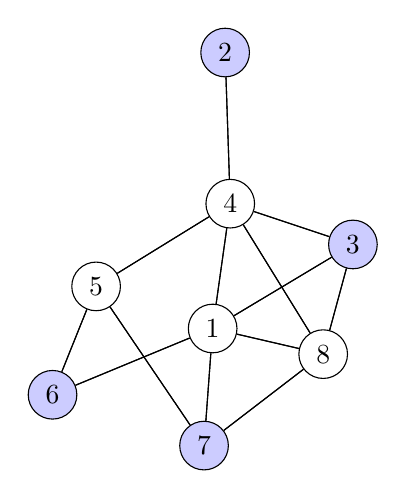
\begin{tikzpicture}[
	every node/.style={draw,circle,fill=white}
	]
	\node  (1) at (0.007009540975573363, -0.5047938530583475)  { 1 };
	\node[fill=blue!20]  (2) at (0.1655944806897962, 3.0)  { 2 };
	\node[fill=blue!20]  (3) at (1.7882499477335903, 0.5624667603559526)  { 3 };
	\node  (4) at (0.2304467971034299, 1.0805731000625989)  { 4 };
	\node  (5) at (-1.473143231371646, 0.02991880959488384)  { 5 };
	\node[fill=blue!20]  (6) at (-2.0265026416974, -1.34637492706497)  { 6 };
	\node[fill=blue!20]  (7) at (-0.10230346491273862, -1.9915902628063684)  { 7 };
	\node  (8) at (1.4106485714793942, -0.8301996270837496)  { 8 };
	\path[draw]  (1) -- (3);
	\path[draw]  (1) -- (4);
	\path[draw]  (1) -- (6);
	\path[draw]  (1) -- (7);
	\path[draw]  (1) -- (8);
	\path[draw]  (2) -- (4);
	\path[draw]  (3) -- (1);
	\path[draw]  (3) -- (4);
	\path[draw]  (3) -- (8);
	\path[draw]  (4) -- (1);
	\path[draw]  (4) -- (2);
	\path[draw]  (4) -- (3);
	\path[draw]  (4) -- (5);
	\path[draw]  (4) -- (8);
	\path[draw]  (5) -- (4);
	\path[draw]  (5) -- (6);
	\path[draw]  (5) -- (7);
	\path[draw]  (6) -- (1);
	\path[draw]  (6) -- (5);
	\path[draw]  (7) -- (1);
	\path[draw]  (7) -- (5);
	\path[draw]  (7) -- (8);
	\path[draw]  (8) -- (1);
	\path[draw]  (8) -- (3);
	\path[draw]  (8) -- (4);
	\path[draw]  (8) -- (7);
\end{tikzpicture}

	\caption{Maximum Independent Set example. The left set is independent, while the right set is a maximum independent set for this graph.}
	\label{fig:mis_example}
\end{figure}

Each constraint $x_i+x_j\leq 1$ prevents adjacent vertices from being selected simultaneously. Together with the binary constraints, these inequalities encode the independent sets of $\G$. Although correct, the edge formulation can have a weak LP relaxation. It can be strengthened using clique inequalities: in any clique $c\subseteq\GV$, at most one vertex can belong to an independent set. Let $\mathcal{C}$ denote a collection of cliques in $\G$; this yields the formulation
\begin{align}
    \label{equ:mis_formulation_cliques}
    (P_\mathrm{MIS}) \Leftrightarrow \left\{
    \begin{array}{lll}
        \max        & \mathds{1}^T x   & \\
        \text{s.t.} & \sum_{i\in c} x_i \leq 1 & \forall c \in \mathcal{C} \\
                    & x \in \{0,1\}^n
    \end{array}
    \right.
\end{align}
The number of cliques can, however, be exponential in $n$, so the full clique formulation is generally not compact. In practice, one may restrict attention to maximal cliques or add violated clique constraints dynamically. This example illustrates a recurring trade-off: stronger formulations may introduce larger or more numerous constraints, which later affects the graphical models built from these constraints.

\subsubsection{Set Cover} 
Given a universe of items $\ITEMS=\{\ITEM_i\}_{i=1}^m$ and a collection of sets $\SCSETS=\{\SCSET_j\}_{j=1}^n$, the objective is to select as few sets as possible while covering every item. We introduce a binary variable $x_j$ for each set $\SCSET_j \in \SCSETS$, and denote by $\SCSETI$ the collection of sets that contain item $\ITEM_i$. The BILP formulation is:
\begin{align}
    \label{equ:sc_formulation}
    (P_\mathrm{SC}) \Leftrightarrow \left\{
    \begin{array}{lll}
        \min        & \mathds{1}^T x   & \\
        \text{s.t.} & \sum_{j:\SCSET_j \in \SCSETI} x_j \geq 1 & \forall 1 \leq i \leq m \\
                    & x \in \{0,1\}^n
    \end{array}
    \right.
\end{align}

Unlike the edge-based MIS formulation, a single SC constraint may involve many variables, since an item can belong to many sets. This makes SC a useful benchmark for feasibility-aware prediction and also foreshadows a scalability issue studied later in the thesis: graphical models built directly from such constraints must handle interactions among many variables at once. Figure~\ref{fig:set_cover_example} illustrates a small SC instance.

\begin{figure}[H]
\centering
\begin{tikzpicture}[scale=1.0]

    % Universe elements
    \node[circle,draw,fill=white,minimum size=7mm] (e1) at (0,0) {1};
    \node[circle,draw,fill=white,minimum size=7mm] (e2) at (2,0) {2};
    \node[circle,draw,fill=white,minimum size=7mm] (e3) at (4,0) {3};
    \node[circle,draw,fill=white,minimum size=7mm] (e4) at (1,-1.8) {4};
    \node[circle,draw,fill=white,minimum size=7mm] (e5) at (3,-1.8) {5};

    % Styles for the sets
    \tikzset{
        setS1/.style={draw=green!60!black,   fill=blue!40,   ellipse, opacity=0.25, inner sep=8pt, line width=2.2pt},
        setS2/.style={draw=red!60!black,    fill=red!50,    ellipse, opacity=0.25, inner sep=8pt},
        setS3/.style={draw=green!60!black, fill=green!50, ellipse, opacity=0.25, inner sep=8pt},
        setS4/.style={draw=green!60!black, fill=orange!70, ellipse, opacity=0.25, inner sep=8pt, line width=2.2pt}
    }

    % Sets as transparent ellipses fitted around the nodes
    \begin{scope}[on background layer]
        % S1 = {1,2,4}
        \node[setS1,fit=(e1)(e2)(e4)] (S1box) {};
        % S2 = {2,3,5}
        \node[setS2,fit=(e2)(e3)] (S2box) {};
        % S3 = {1,4,5}
        \node[setS3,fit=(e4)(e5)] (S3box) {};
        % S4 = {3,4}
        \node[setS4,rotate=-30,fit=(e3)(e5)]     (S4box) {};
    \end{scope}

    % Labels for the sets (placed near ellipse anchors)
    \node[blue!70!black,anchor=south west]  at (S1box.north west) {\scriptsize $S_1=\{1,2,4\}$};
    \node[red!80!black,anchor=south east]   at (S2box.north east) {\scriptsize $S_2=\{2,3\}$};
    \node[green!70!black,anchor=north west] at (S3box.south west) {\scriptsize $S_3=\{4,5\}$};
    \node[orange!80!black,anchor=north east]at (S4box.south east) {\scriptsize $S_4=\{3,5\}$};

\end{tikzpicture}
\caption{Set covering illustration with sets $S_1,\dots,S_4$ covering the universe $U=\{1,2,3,4,5\}$. The minimal set cover is $\{ S_1, S_4 \}$.}
\label{fig:set_cover_example}
\end{figure}


\subsection{Summary: ILPs as structured prediction inputs}

This section introduced BILP formulations, the classical solver context, and the graph representation used to encode ILP structure. The key point for the remainder of the thesis is that feasibility constraints couple the binary decision variables: predicting each variable independently is generally insufficient to obtain a valid solution. The variable-constraint graph provides a natural input representation for learning models, while later sections will show how related graphical structures can represent interactions between solution variables.

The next sections build on this view by introducing neural models for structured prediction and Markov Random Fields for representing and inferring over coupled solution variables. The high-arity constraints that arise in problems such as Set Cover will later motivate approximate graphical parameterizations.

\section{Machine Learning and Deep Learning}
\label{sec:ml_intro}

Machine Learning (ML), and in particular \emph{Deep Learning} (DL), is the field of study concerned with designing and training parameterized mathematical models to perform tasks through experience rather than explicit programming \cite{heaton_ian_2018,noauthor_pattern_2007}. Learning algorithms can be categorized in various ways, two of the most prominent paradigms being \emph{supervised} and \emph{unsupervised} learning. 

In general, a machine learning model is a parameterized function 
\begin{equation}
    f_{\theta} : \mathcal{X} \rightarrow \mathcal{Y},
\end{equation}
where $\mathcal{X}$ denotes the input domain (often referred to as the \emph{feature space}), $\mathcal{Y}$ the output domain (labels or targets), and $\theta \in \Theta$ the set of \emph{trainable parameters}. The model is evaluated according to a task-specific \emph{loss function} 
\begin{equation}
    \mathcal{L} : \Theta \times \mathcal{X} \rightarrow \mathbb{R},
\end{equation}
which measures the ability of the model with parameters $\theta$ to perform the desired task on an input $x \in \mathcal{X}$. For convenience, we assume that smaller values of $\mathcal{L}$ correspond to better performance. The goal of the training process is to find parameters $\theta^*$ that minimize this loss, typically formulated as the optimization problem
\begin{equation}
    \label{equ:training_task}
    \theta^* = \argmin_{\theta \in \Theta} \, \mathbb{E}_{x \sim \mathcal{D}} \, \mathcal{L}(\theta, x),
\end{equation}
where $\mathcal{D}$ denotes the data distribution over the input space.

In \emph{supervised learning}, the dataset $\mathcal{D}$ provides labeled examples $(x, y)$, allowing direct estimation of $\theta^*$ by gradient-based optimization (e.g., stochastic gradient descent). In contrast, \emph{unsupervised learning} seeks to discover hidden structure in unlabeled data, often by optimizing surrogate objectives such as likelihoods or reconstruction errors. Many modern frameworks extend these two paradigms to encompass reinforcement learning, self-supervised learning, and generative modeling, broadening the scope of ML beyond prediction toward reasoning and structured decision-making \cite{lecun_deep_2015}.

In this work, we focus on learning paradigms where ML models are used to approximate or guide optimization processes, often by learning mappings from structured problem instances to high-quality solutions or to efficient inference strategies. Such approaches are particularly relevant in the context of combinatorial optimization and probabilistic graphical models, as discussed in later sections (see \S\ref{sec:mrf_intro} and \S\ref{sec:co_intro}).


\subsection{Supervised Learning}
\label{sec:supervised_learning}

Supervised learning refers to the class of learning strategies in which the \emph{ground truth} or target value is available during training. Formally, we assume access to a dataset of input–output pairs 
\begin{equation}
    \mathcal{D} = \{(x_i, y_i)\}_{i=1}^{N}, \quad x_i \in \mathcal{X}, \; y_i \in \mathcal{Y},
\end{equation}
where each input $x_i$ is associated with a corresponding label $y_i$ representing the correct or desired outcome. The objective is to learn a parameterized function $f_{\theta} : \mathcal{X} \rightarrow \mathcal{Y}$ capable of producing predictions $\hat{y} = f_{\theta}(x)$ that generalize well to unseen data drawn from the same underlying distribution $\mathcal{D}$.

By quantifying the discrepancy between the predicted outcome $\hat{y}$ and the ground truth $y$, it becomes possible to define a \emph{loss function} $\mathcal{L}_{\text{sup}} : \Theta \times \mathcal{X} \times \mathcal{Y} \rightarrow \mathbb{R}$ that measures model performance on each training example. The learning problem is then formulated as minimizing the expected loss over the data distribution:
\begin{equation}
    \label{equ:supervised_learning}
    \theta^* = \argmin_{\theta \in \Theta} \, \mathbb{E}_{(x,y) \sim \mathcal{D}} \left[ \mathcal{L}_{\text{sup}}(\theta, x, y) \right].
\end{equation}

In practice, this expectation is approximated by the empirical average over the training set:
\begin{equation}
    \widehat{\mathcal{L}}_{\text{sup}}(\theta) = \frac{1}{N} \sum_{i=1}^{N} \mathcal{L}_{\text{sup}}(\theta, x_i, y_i).
\end{equation}

The form of $\mathcal{L}_{\text{sup}}$ depends on the prediction task:
\begin{itemize}
    \item In \emph{regression} tasks, the model predicts continuous quantities and typical losses include the squared error $\mathcal{L}_{\text{sup}} = \| f_{\theta}(x) - y \|^2$ or the mean absolute error.
    \item In \emph{classification} tasks, where the label $y$ belongs to a discrete set of classes, the loss commonly takes the form of the negative log-likelihood or cross-entropy:
    \begin{equation}
        \mathcal{L}_{\text{sup}}(\theta, x, y) = - \log p_{\theta}(y|x),
    \end{equation}
    where $p_{\theta}(y|x)$ denotes the model’s predicted probability for the correct class.
\end{itemize}

Supervised learning thus reduces to a parameter optimization problem, where $\theta$ is iteratively updated to minimize $\widehat{\mathcal{L}}_{\text{sup}}(\theta)$ using stochastic gradient descent or one of its many variants \cite{goodfellow_deep_2016,kingma_adam_2014}. When the learned parameters generalize beyond the training data, the model effectively captures an underlying mapping between inputs and outputs, a property central to most modern applications of deep learning \cite{vapnik_nature_2000,bishop_pattern_2006}.

\subsection{Unsupervised Learning}
\label{sec:unsupervised_learning}

Unsupervised learning encompasses learning paradigms in which no explicit ground-truth labels or target outputs are provided during training. Instead, the objective is to discover latent structures, dependencies, or representations within the data itself \cite{bishop_pattern_2006,goodfellow_deep_2016}. Formally, given a dataset of unlabeled examples 
\begin{equation}
    \mathcal{D} = \{ x_i \}_{i=1}^{N}, \quad x_i \in \mathcal{X},
\end{equation}
the goal is to learn parameters $\theta$ that optimize a self-consistency criterion defined by a loss function $\mathcal{L}_{\text{unsup}} : \Theta \times \mathcal{X} \rightarrow \mathbb{R}$,
\begin{equation}
    \label{equ:unsupervised_learning}
    \theta^* = \argmin_{\theta \in \Theta} \, \mathbb{E}_{x \sim \mathcal{D}} \left[ \mathcal{L}_{\text{unsup}}(\theta, x) \right].
\end{equation}

The precise form of $\mathcal{L}_{\text{unsup}}$ depends on the learning objective. Common unsupervised frameworks include:

\paragraph{1. Representation learning and dimensionality reduction.}
Methods such as \emph{Principal Component Analysis (PCA)} \cite{jolliffe_principal_2010}, \emph{autoencoders} \cite{hinton_reducing_2006}, and their probabilistic extensions aim to learn low-dimensional latent representations $z = g_{\theta}(x)$ that capture the salient structure of the data. In an autoencoder, for instance, the model is composed of an encoder–decoder pair $(g_{\theta}, d_{\theta})$ trained to minimize the reconstruction error:
\begin{equation}
    \mathcal{L}_{\text{rec}}(\theta, x) = \| d_{\theta}(g_{\theta}(x)) - x \|^2,
\end{equation}
thus encouraging the latent code $z$ to capture the essential variability in $\mathcal{X}$ while discarding noise and redundancy \cite{ hinton_reducing_2006,kingma_auto-encoding_2022}.

\paragraph{2. Density estimation and probabilistic modeling.}
Another key class of unsupervised methods seeks to model the underlying data distribution $p_{\theta}(x)$ directly. Training such models typically involves maximizing the likelihood of the observed data, or equivalently, minimizing the negative log-likelihood loss:
\begin{equation}
    \mathcal{L}_{\text{nll}}(\theta, x) = - \log p_{\theta}(x).
\end{equation}
Examples include probabilistic graphical models such as Markov Random Fields (MRFs) and Conditional Random Fields (CRFs), as well as modern generative models like Variational Autoencoders (VAEs) \cite{kingma_introduction_2019} and Generative Adversarial Networks (GANs) \cite{goodfellow_generative_2014}. These models can capture complex dependencies between variables and generate realistic new samples from learned distributions.

\paragraph{3. Clustering and self-organization.}
In clustering-based approaches, the learning process groups similar samples together according to an implicit or explicit similarity measure. Classical
algorithms include $k$-means, Gaussian mixture models, and spectral clustering \cite{macqueen_methods_1967,dempster_maximum_1977,ng_spectral_2001}. In the neural setting, differentiable clustering losses or contrastive objectives are often employed to encourage representation spaces where semantically similar samples are close together \cite{oord_representation_2019,chen_simple_2020}.

Overall, unsupervised learning provides a foundation for learning useful data representations and priors that can later be exploited in semi-supervised, transfer, or reinforcement learning contexts. In this work, it plays a key role in formulating models that learn from problem structure—rather than explicit supervision—especially in the context of probabilistic graphical models and combinatorial optimization, where ground-truth solutions are expensive or unavailable.


\subsection{Generative Models and Denoising Objectives}

Generative models aim to learn a probability distribution over the data, rather than directly predicting a single deterministic output. In the conditional setting considered throughout this thesis, an input instance $x \in \mathcal{X}$ may be associated with multiple valid or high-quality outputs $y \in \mathcal{Y}$. This is particularly relevant in combinatorial optimization, where a problem instance can admit several near-optimal solutions with different structures. Instead of returning a single prediction, a generative model defines a conditional distribution over possible outputs and obtains predictions by sampling from this distribution (see Figure~\ref{fig:conditional_generative_graph}).

Formally, we view input-output pairs as realizations of random variables $X$ and $Y$. The goal is to approximate the conditional distribution
\begin{equation}
    p(y \mid x) = \mathbb{P}\left[ Y = y \mid X = x \right],
\end{equation}
where $x$ denotes the observed input instance and $y$ denotes a target output, such as a feasible solution or an optimal assignment.

In practice, the true conditional distribution $p(y \mid x)$ is unknown and must be approximated by a parameterized model. We denote this approximation by $p_\Theta(y \mid x)$, where $\Theta$ are learned parameters. In some models, the input $x$ is first mapped to the parameters of an output distribution, for example through a neural network $\Theta = f_\theta(x)$, yielding a distribution $p_\Theta(y)$. Predictions can then be obtained by sampling
\begin{equation}
    y \sim p_\Theta(\cdot \mid x),
\end{equation}
or by selecting high-probability outputs according to the learned distribution.

Different families of generative models mainly differ in how they parameterize this distribution and in the training objective used to match it to the data distribution. Examples include maximum-likelihood objectives, variational objectives, adversarial objectives, denoising objectives, and, more recently, diffusion and flow-matching objectives. In the remainder of this section, we focus on denoising-based generative models, since they provide the conceptual basis for the diffusion and flow-based decoding methods studied later in this thesis.

\begin{figure}[t]
\centering
\begin{tikzpicture}[
    font=\small,
    >=Latex,
    panel/.style={
        rounded corners=8pt,
        draw=#1,
        fill=#1!6,
        line width=0.9pt,
        inner sep=6pt
    },
    stagecircle/.style={
        circle,
        fill=#1,
        text=white,
        font=\bfseries,
        minimum size=7mm,
        inner sep=0pt
    },
    arrow/.style={
        -{Latex[length=3mm,width=2mm]},
        line width=1.1pt,
        draw=blue!55!black
    },
    dottedarrow/.style={
        -{Latex[length=3mm,width=2mm]},
        line width=1.1pt,
        draw=blue!55!black,
        dotted
    },
    itemrow/.style={
        rounded corners=3pt,
        draw=gray!30,
        fill=white,
        minimum height=6mm,
        inner sep=2pt
    },
    probbar/.style={
        draw=none,
        fill=green!60!black,
        rounded corners=1pt
    },
    nodecircle/.style={
        circle,
        draw=blue!50!black,
        fill=blue!15,
        minimum size=3.5mm,
        inner sep=0pt
    },
    hiddennode/.style={
        circle,
        draw=green!50!black,
        fill=green!25,
        minimum size=3.5mm,
        inner sep=0pt
    },
    outputnode/.style={
        circle,
        draw=purple!60!black,
        fill=purple!20,
        minimum size=3.5mm,
        inner sep=0pt
    }
]

% =========================================================
% Colors
% =========================================================
\definecolor{TitleColor}{RGB}{10,25,70}
\definecolor{PurplePanel}{RGB}{130,100,200}
\definecolor{BluePanel}{RGB}{65,130,200}
\definecolor{GreenPanel}{RGB}{40,135,85}
\definecolor{OrangePanel}{RGB}{220,145,25}

\definecolor{NodeA}{RGB}{220,50,47}
\definecolor{NodeB}{RGB}{38,139,210}
\definecolor{NodeC}{RGB}{133,153,0}
\definecolor{NodeD}{RGB}{181,137,0}
\definecolor{NodeE}{RGB}{108,113,196}

% =========================================================
% Panel coordinates
% =========================================================
\coordinate (P1) at (-6.0,0);
\coordinate (P2) at (-2.0,0);
\coordinate (P3) at ( 2.1,0);
\coordinate (P4) at ( 6.1,0);

% =========================================================
% Stage badges and headings (moved higher)
% =========================================================
% \node[stagecircle=PurplePanel] at ($(P1)+(0,2.65)$) {1};
% \node[font=\bfseries\large, text=TitleColor] at ($(P1)+(0,2.25)$) {Input};

% \node[stagecircle=BluePanel] at ($(P2)+(0,2.65)$) {2};
% \node[font=\bfseries\large, text=TitleColor] at ($(P2)+(0,2.25)$) {Model};

% \node[stagecircle=GreenPanel] at ($(P3)+(0,2.65)$) {3};
% \node[font=\bfseries\large, text=TitleColor] at ($(P3)+(0,2.25)$) {Distribution};

% \node[stagecircle=OrangePanel] at ($(P4)+(0,2.65)$) {4};
% \node[font=\bfseries\large, text=TitleColor] at ($(P4)+(0,2.25)$) {Sample};

% =========================================================
% Stage 1: Input graph
% =========================================================
\node[panel=PurplePanel, minimum width=3.0cm, minimum height=4.3cm, anchor=center] (inputpanel) at (P1) {};
\node[font=\bfseries, text=TitleColor] at ($(P1)+(0,1.75)$) {Input};

\begin{scope}[shift={(P1)}, scale=0.92]
    % Graph nodes
    \node[circle, draw=black, fill=NodeA!75, minimum size=7mm, inner sep=0pt] (gA) at (-0.55,0.95) {};
    \node[circle, draw=black, fill=NodeB!75, minimum size=7mm, inner sep=0pt] (gB) at (0.55,1.05) {};
    \node[circle, draw=black, fill=NodeC!75, minimum size=7mm, inner sep=0pt] (gC) at (-0.95,-0.05) {};
    \node[circle, draw=black, fill=NodeD!75, minimum size=7mm, inner sep=0pt] (gD) at (0.05,-0.15) {};
    \node[circle, draw=black, fill=NodeE!75, minimum size=7mm, inner sep=0pt] (gE) at (0.95,-0.85) {};

    % Graph edges
    \draw[thick, gray!70] (gA) -- (gB);
    \draw[thick, gray!70] (gA) -- (gC);
    \draw[thick, gray!70] (gA) -- (gD);
    \draw[thick, gray!70] (gB) -- (gD);
    \draw[thick, gray!70] (gC) -- (gD);
    \draw[thick, gray!70] (gD) -- (gE);

    % Labels
    \node[font=\scriptsize] at (gA) {$1$};
    \node[font=\scriptsize] at (gB) {$2$};
    \node[font=\scriptsize] at (gC) {$3$};
    \node[font=\scriptsize] at (gD) {$4$};
    \node[font=\scriptsize] at (gE) {$5$};
\end{scope}

\node[font=\Large] at ($(P1)+(0,-1.5)$) {$x$};

% =========================================================
% Stage 2: Model panel
% =========================================================
\node[panel=BluePanel, minimum width=3.5cm, minimum height=4.3cm] (modelpanel) at (P2) {};
\node[font=\bfseries, text=TitleColor] at ($(P2)+(0,1.75)$) {Neural network};

\begin{scope}[shift={(P2)}, scale=0.88]
    % Neural network nodes
    \foreach \i/\yy in {1/0.78,2/0.33,3/-0.12,4/-0.57}{
        \node[nodecircle] (in\i) at (-0.95,\yy) {};
    }
    \foreach \i/\yy in {1/0.82,2/0.37,3/-0.08,4/-0.53}{
        \node[hiddennode] (hA\i) at (-0.25,\yy) {};
        \node[hiddennode] (hB\i) at (0.42,\yy) {};
    }
    \foreach \i/\yy in {1/0.58,2/0.02,3/-0.54}{
        \node[outputnode] (out\i) at (1.02,\yy) {};
    }

    \foreach \i in {1,2,3,4}{
        \foreach \j in {1,2,3,4}{
            \draw[blue!45!black, line width=0.35pt] (in\i) -- (hA\j);
            \draw[blue!45!black, line width=0.35pt] (hA\i) -- (hB\j);
        }
    }
    \foreach \i in {1,2,3,4}{
        \foreach \j in {1,2,3}{
            \draw[blue!45!black, line width=0.35pt] (hB\i) -- (out\j);
        }
    }
\end{scope}

\node[font=\Large] at ($(P2)+(0,-1.45)$) {$p_\theta(y \mid x)$};

% =========================================================
% Stage 3: Distribution panel
% =========================================================
\node[panel=GreenPanel, minimum width=3.25cm, minimum height=4.3cm] (distpanel) at (P3) {};
\node[font=\bfseries, text=TitleColor, align=center] at ($(P3)+(0,1.48)$) {Node selection\\probabilities};

\begin{scope}[shift={(P3)}, scale=0.88]
    \foreach \y/\name/\col/\prob/\barlen in {
        0.82/Node 1/NodeA/0.82/1.05,
        0.35/Node 2/NodeB/0.21/0.27,
        -0.12/Node 3/NodeC/0.73/0.92,
        -0.59/Node 4/NodeD/0.15/0.20,
        -1.06/Node 5/NodeE/0.78/0.98
    }{
        \node[itemrow, minimum width=2.65cm, minimum height=3.8mm] at (0,\y) {};
        \node[circle, draw=black, fill=\col!75, minimum size=2.8mm, inner sep=0pt] at (-1.02,\y) {};
        %\node[anchor=west, font=\scriptsize] at (-0.82,\y) {\name};
        \draw[probbar] (0.08,\y-0.08) rectangle ++(\barlen,0.16);
        %\node[anchor=east, font=\scriptsize, text=GreenPanel!80!black] at (1.25,\y) {\prob};
    }
\end{scope}

%\node[font=\large] at ($(P3)+(0,-1.55)$) {$y \sim p_\theta(\cdot \mid x)$};

% =========================================================
% Stage 4: Sampled solution graph
% =========================================================
\node[panel=OrangePanel, minimum width=3.0cm, minimum height=4.3cm] (samplepanel) at (P4) {};
\node[font=\bfseries, text=TitleColor] at ($(P4)+(0,1.75)$) {Sample};

\begin{scope}[shift={(P4)}, scale=0.92]
    % Faded original graph
    \node[circle, draw=gray!60, fill=NodeA!20, minimum size=7mm, inner sep=0pt] (sA) at (-0.55,0.95) {};
    \node[circle, draw=gray!60, fill=gray!15, minimum size=7mm, inner sep=0pt] (sB) at (0.55,1.05) {};
    \node[circle, draw=gray!60, fill=NodeC!25, minimum size=7mm, inner sep=0pt] (sC) at (-0.95,-0.05) {};
    \node[circle, draw=gray!60, fill=gray!15, minimum size=7mm, inner sep=0pt] (sD) at (0.05,-0.15) {};
    \node[circle, draw=gray!60, fill=NodeE!25, minimum size=7mm, inner sep=0pt] (sE) at (0.95,-0.85) {};

    \draw[thick, gray!35] (sA) -- (sB);
    \draw[thick, gray!35] (sA) -- (sC);
    \draw[thick, gray!35] (sA) -- (sD);
    \draw[thick, gray!35] (sB) -- (sD);
    \draw[thick, gray!35] (sC) -- (sD);
    \draw[thick, gray!35] (sD) -- (sE);

    % Highlight sampled nodes only
    \draw[line width=1.2pt, black] (sA) circle (3.6mm);
    \draw[line width=1.2pt, black] (sC) circle (3.6mm);
    \draw[line width=1.2pt, black] (sE) circle (3.6mm);

    \node[font=\scriptsize] at (sA) {$1$};
    \node[font=\scriptsize, text=gray!60] at (sB) {$2$};
    \node[font=\scriptsize] at (sC) {$3$};
    \node[font=\scriptsize, text=gray!60] at (sD) {$4$};
    \node[font=\scriptsize] at (sE) {$5$};
\end{scope}

\node[font=\large] at ($(P4)+(0,-1.5)$)
{$\{1,3,5\}$};

% =========================================================
% Arrows between stages
% =========================================================
\draw[arrow] ($(inputpanel.east)+(0.10,0)$) -- ($(modelpanel.west)+(-0.10,0)$);
\draw[arrow] ($(modelpanel.east)+(0.10,0)$) -- ($(distpanel.west)+(-0.10,0)$);
\draw[dottedarrow] ($(distpanel.east)+(0.10,0)$) -- ($(samplepanel.west)+(-0.10,0)$)
    node[midway, above, font=\scriptsize\itshape, text=blue!55!black] {};

\end{tikzpicture}
\caption{Illustration of conditional generative modeling for a combinatorial optimization problem. A graph-structured input instance is processed by a neural network, which predicts selection probabilities for the nodes. A candidate solution is then obtained by sampling a subset of nodes from the predicted distribution.}
\label{fig:conditional_generative_graph}
\end{figure}

\paragraph{Denoising-based generative modeling.}

A central idea in modern generative modeling is to learn how to recover structured data from corrupted observations. Instead of directly learning to sample from the data distribution, denoising-based methods define a corruption process that progressively perturbs a clean target $y$ into a noisy version $\tilde{y}$. A model is then trained to invert this process, either by predicting the original clean sample, the noise that was added, or an update direction that moves the corrupted sample closer to the data distribution.

Let $y \in \mathcal{Y}$ denote a clean target output, such as an optimal or high-quality solution of a combinatorial optimization problem. A corruption process defines a conditional distribution
\begin{equation}
    q(\tilde{y} \mid y, t),
\end{equation}
where $t$ denotes the noise level or time index. For small values of $t$, the corrupted sample $\tilde{y}$ remains close to the original target, while for large values of $t$ it may contain little information about $y$. The learning problem consists in training a model that, given the corrupted sample $\tilde{y}$, the input instance $x$, and the noise level $t$, predicts how to recover information about the clean output:
\begin{equation}
    D_\theta(x, \tilde{y}, t) \approx y.
\end{equation}
Equivalently, depending on the formulation, the model may predict the perturbation applied to $y$, or a direction in the output space that transforms $\tilde{y}$ toward a clean sample.

\begin{figure}[t]
\centering
\begin{tikzpicture}[
    font=\small,
    >=Latex,
    arrow/.style={
        -{Latex[length=3mm,width=2mm]},
        line width=1.1pt,
        draw=blue!60!black
    },
    panel/.style={
        rounded corners=8pt,
        line width=0.9pt,
        inner sep=6pt
    },
    stagebadge/.style={
        circle,
        minimum size=7mm,
        inner sep=0pt,
        font=\bfseries,
        text=white
    },
    clean/.style={
        circle,
        draw=black,
        line width=0.8pt,
        minimum size=7mm,
        inner sep=0pt
    },
    noisy/.style={
        circle,
        draw=gray!70,
        fill=gray!30,
        line width=0.8pt,
        minimum size=7mm,
        inner sep=0pt
    },
    inactive/.style={
        circle,
        draw=gray!60,
        fill=white,
        line width=0.8pt,
        minimum size=7mm,
        inner sep=0pt
    },
    nninput/.style={
        circle,
        draw=blue!55!black,
        fill=blue!15,
        minimum size=3.8mm,
        inner sep=0pt
    },
    nnhidden/.style={
        circle,
        draw=green!50!black,
        fill=green!25,
        minimum size=3.8mm,
        inner sep=0pt
    },
    nnoutput/.style={
        circle,
        draw=purple!60!black,
        fill=purple!20,
        minimum size=3.8mm,
        inner sep=0pt
    }
]

% -------------------------------------------------
% Colors
% -------------------------------------------------
\definecolor{TitleColor}{RGB}{10,25,70}
\definecolor{PurplePanel}{RGB}{130,100,200}
\definecolor{BluePanel}{RGB}{65,130,200}
\definecolor{GreenPanel}{RGB}{40,135,85}

\definecolor{NodeSel}{RGB}{166,206,57}   % selected node
\definecolor{NodeAlt}{RGB}{102,194,255}  % alternate highlight
\definecolor{NodeWarn}{RGB}{255,180,70}  % optional accent

% -------------------------------------------------
% Coordinates of the three stages
% -------------------------------------------------
\coordinate (P1) at (-4.8,0);
\coordinate (P2) at (0,0);
\coordinate (P3) at (4.8,0);

% -------------------------------------------------
% Headings
% -------------------------------------------------
% \node[stagebadge, fill=PurplePanel] at ($(P1)+(0,2.5)$) {1};
% \node[font=\bfseries\large, text=TitleColor] at ($(P1)+(0,2.1)$) {Noisy input};

% \node[stagebadge, fill=BluePanel] at ($(P2)+(0,2.5)$) {2};
% \node[font=\bfseries\large, text=TitleColor] at ($(P2)+(0,2.1)$) {Prediction};

% \node[stagebadge, fill=GreenPanel] at ($(P3)+(0,2.5)$) {3};
% \node[font=\bfseries\large, text=TitleColor] at ($(P3)+(0,2.1)$) {Denoised output};

% -------------------------------------------------
% Panel 1 : Noisy solution
% -------------------------------------------------
\node[panel, draw=PurplePanel, fill=PurplePanel!6, minimum width=3.3cm, minimum height=4.1cm] (noisypanel) at (P1) {};

\node[font=\bfseries, text=TitleColor] at ($(P1)+(0,1.75)$) {Noise};

\begin{scope}[shift={(P1)}, scale=0.95]
    % nodes
    \node[clean, fill=NodeSel!85] (a1) at (-0.75, 0.95) {};
    \node[noisy]               (a2) at ( 0.35, 1.05) {};
    \node[clean, fill=NodeSel!85] (a3) at (-1.05,-0.05) {};
    \node[noisy]               (a4) at ( 0.10,-0.18) {};
    \node[inactive]            (a5) at ( 0.95,-0.75) {};
    \node[inactive]            (a6) at (-0.20,-0.95) {};

    % edges
    \draw[thick, gray!65] (a1) -- (a2);
    \draw[thick, gray!65] (a1) -- (a3);
    \draw[thick, gray!65] (a1) -- (a4);
    \draw[thick, gray!65] (a2) -- (a4);
    \draw[thick, gray!65] (a3) -- (a4);
    \draw[thick, gray!65] (a4) -- (a5);
    \draw[thick, gray!65] (a3) -- (a6);

    % labels
    \node[font=\scriptsize] at (a1) {$1$};
    \node[font=\scriptsize, text=gray!60!black] at (a2) {?};
    \node[font=\scriptsize] at (a3) {$3$};
    \node[font=\scriptsize, text=gray!60!black] at (a4) {?};
    \node[font=\scriptsize, text=gray!70!black] at (a5) {$5$};
    \node[font=\scriptsize, text=gray!70!black] at (a6) {$6$};
\end{scope}

\node[align=center] at ($(P1)+(0,-1.8)$)
{Noisy solution $\tilde y$};

% -------------------------------------------------
% Panel 2 : Denoising model
% -------------------------------------------------
\node[panel, draw=BluePanel, fill=BluePanel!6, minimum width=3.7cm, minimum height=4.1cm] (modelpanel) at (P2) {};
\node[font=\bfseries, text=TitleColor] at ($(P2)+(0,1.75)$) {Denoising model};

\begin{scope}[shift={(P2)}, scale=0.9]
    % network
    \foreach \i/\yy in {1/0.75,2/0.25,3/-0.25,4/-0.75}{
        \node[nninput] (i\i) at (-0.95,\yy) {};
    }
    \foreach \i/\yy in {1/0.9,2/0.3,3/-0.3,4/-0.9}{
        \node[nnhidden] (h\i) at (0,\yy) {};
    }
    \foreach \i/\yy in {1/0.5,2/0.0,3/-0.5}{
        \node[nnoutput] (o\i) at (0.95,\yy) {};
    }

    \foreach \u in {1,2,3,4}{
        \foreach \v in {1,2,3,4}{
            \draw[blue!50!black, line width=0.35pt] (i\u) -- (h\v);
        }
    }
    \foreach \u in {1,2,3,4}{
        \foreach \v in {1,2,3}{
            \draw[blue!50!black, line width=0.35pt] (h\u) -- (o\v);
        }
    }
\end{scope}

\node[align=center] at ($(P2)+(0,-1.8)$)
{$\hat y = f_\theta(\tilde y, x)$};

% -------------------------------------------------
% Panel 3 : Denoised output
% -------------------------------------------------
\node[panel, draw=GreenPanel, fill=GreenPanel!6, minimum width=3.3cm, minimum height=4.1cm] (cleanpanel) at (P3) {};
\node[font=\bfseries, text=TitleColor] at ($(P3)+(0,1.75)$) {Denoised};

\begin{scope}[shift={(P3)}, scale=0.95]
    % nodes
    \node[clean, fill=NodeSel!85] (b1) at (-0.75, 0.95) {};
    \node[inactive]               (b2) at ( 0.35, 1.05) {};
    \node[clean, fill=NodeSel!85] (b3) at (-1.05,-0.05) {};
    \node[inactive]               (b4) at ( 0.10,-0.18) {};
    \node[inactive]               (b5) at ( 0.95,-0.75) {};
    \node[clean, fill=NodeSel!85] (b6) at (-0.20,-0.95) {};

    % edges
    \draw[thick, gray!65] (b1) -- (b2);
    \draw[thick, gray!65] (b1) -- (b3);
    \draw[thick, gray!65] (b1) -- (b4);
    \draw[thick, gray!65] (b2) -- (b4);
    \draw[thick, gray!65] (b3) -- (b4);
    \draw[thick, gray!65] (b4) -- (b5);
    \draw[thick, gray!65] (b3) -- (b6);

    % labels
    \node[font=\scriptsize] at (b1) {$1$};
    \node[font=\scriptsize, text=gray!70!black] at (b2) {$2$};
    \node[font=\scriptsize] at (b3) {$3$};
    \node[font=\scriptsize, text=gray!70!black] at (b4) {$4$};
    \node[font=\scriptsize, text=gray!70!black] at (b5) {$5$};
    \node[font=\scriptsize] at (b6) {$6$};
\end{scope}

\node[align=center] at ($(P3)+(0,-1.8)$)
{Solution $\hat y$};

% -------------------------------------------------
% Arrows
% -------------------------------------------------
\draw[arrow] ($(noisypanel.east)+(0.08,0)$) -- ($(modelpanel.west)+(-0.08,0)$);
\draw[arrow] ($(modelpanel.east)+(0.08,0)$) -- ($(cleanpanel.west)+(-0.08,0)$);


\end{tikzpicture}
\caption{Illustration of denoising for graph-structured solutions. Starting from a corrupted or partially masked solution $\tilde y$, a prediction model infers corrected node assignments and outputs a denoised solution $\hat y$. Gray nodes indicate noisy or uncertain values.}
\label{fig:graph_denoising_illustration}
\end{figure}

This denoising view is especially natural for structured prediction. In many problems, the output is not a single scalar label but a structured object composed of many dependent decisions. In combinatorial optimization, for example, a solution may be represented by a binary vector $y \in \{0,1\}^n$, where each component corresponds to the value of a decision variable. Corrupting such a solution can be interpreted as randomly masking, flipping, or relaxing some of its variables. The denoising model must then learn how local and global dependencies between variables constrain the reconstruction of a valid or high-quality solution.

A common training objective is to minimize a reconstruction loss between the model prediction and the clean target. For example, when the model predicts the original solution, one may use
\begin{equation}
    \mathcal{L}_{\mathrm{denoise}}(\theta)
    =
    \mathbb{E}_{(x,y),t,\tilde{y}}
    \left[
        \ell\left(D_\theta(x,\tilde{y},t), y\right)
    \right],
\end{equation}
where $\tilde{y} \sim q(\cdot \mid y,t)$ and $\ell$ is a suitable loss function, such as a cross-entropy loss for discrete variables or a squared error loss for continuous relaxations. The model is therefore trained on many reconstruction tasks of varying difficulty, ranging from lightly corrupted samples to highly noisy ones.

At inference time, denoising-based generative models reverse the corruption process. Starting from a noisy or partially initialized sample, the learned denoising model is applied iteratively to produce increasingly structured outputs. This procedure can be interpreted as a learned refinement process: each denoising step uses the instance information $x$, the current candidate solution, and the noise level to move the sample toward the learned solution distribution.

In the context of this thesis, this perspective is useful because it connects generative modeling with solution construction. Rather than predicting each variable independently in a single forward pass, a denoising model defines a dynamics over candidate solutions. This makes it possible to progressively refine a noisy assignment into a feasible or high-quality solution, while potentially capturing dependencies between variables through the architecture used to parameterize the denoising function.

This general principle underlies both diffusion models, which learn to reverse a stochastic noising process, and flow-based formulations, which learn a deterministic or approximately deterministic transformation from a simple initial distribution toward the data distribution.

\paragraph{Flow matching and velocity prediction models.}

Flow matching is a generative modeling framework in which the model learns a time-dependent transformation between a simple source distribution and the data distribution. Instead of learning a reverse stochastic denoising chain, as in diffusion models, flow matching trains a neural network to predict a velocity field that transports samples from an initial distribution toward the target distribution.

Let $y_0 \sim p_0$ denote a sample from a simple source distribution, such as Gaussian noise, and let $y_1 \sim p_{\mathrm{data}}$ denote a target data sample. Flow matching defines a family of intermediate states $y_t$ for $t \in [0,1]$ that interpolate between $y_0$ and $y_1$. A common choice is the linear interpolation path
\begin{equation}
    y_t = (1-t)y_0 + t y_1.
\end{equation}
Along this path, the corresponding target velocity is
\begin{equation}
    u_t = \frac{d y_t}{dt} = y_1 - y_0.
\end{equation}
The learning problem is then to train a parameterized model $v_\theta$ to predict this velocity from the current state and time:
\begin{equation}
    v_\theta(y_t,t) \approx u_t.
\end{equation}
In a conditional setting, where generation depends on an input instance $x$, the model is instead written as
\begin{equation}
    v_\theta(x_t,t,x) \approx u_t.
\end{equation}
For example, in combinatorial optimization, $x$ may represent the optimization instance and $y_1$ may represent an optimal or high-quality solution.

The standard flow matching objective takes the form
\begin{equation}
    \mathcal{L}_{\mathrm{FM}}(\theta)
    =
    \mathbb{E}_{t,y_0,y_1}
    \left[
        \left\|
            v_\theta(y_t,t,x) - u_t
        \right\|_2^2
    \right],
\end{equation}
where $t$ is sampled from $[0,1]$, $y_0$ is sampled from the source distribution, $y_1$ is sampled from the data distribution, and $y_t$ is obtained from the chosen interpolation path. The model is therefore trained by supervised regression onto a known velocity target.

Once the velocity field has been learned, samples can be generated by starting from $y_0 \sim p_0$ and solving the ordinary differential equation (see Algorithm~\ref{alg:flow_sampling})
\begin{equation}
    \frac{d y_t}{dt} = v_\theta(y_t,t,x),
    \qquad y_0 \sim p_0.
\end{equation}
The endpoint $y_1$ of this trajectory is then expected to follow the learned data distribution. In practice, this ODE is solved numerically using a finite number of integration steps. Compared with diffusion models, this formulation often leads to a more direct generative procedure, since the model predicts a deterministic direction of motion rather than the parameters of a stochastic reverse transition.

\begin{algorithm}[t]
\caption{Sample generation with a learned velocity field}
\label{alg:flow_sampling}
\DontPrintSemicolon

\KwIn{
    Problem instance $x$;
    learned velocity field $v_\theta$;
    source distribution $p_0$;
    number of integration steps $K$;
    decoding operator $\mathcal{D}$
}
\KwOut{
    Discrete candidate solution $\hat{y}$
}

Sample an initial state $y^{(0)} \sim p_0$\;
Set $\Delta t \leftarrow 1/K$\;

\For{$k = 0,\ldots,K-1$}{
    Set $t_k \leftarrow k \Delta t$\;
    
    Predict the velocity $\hat{u}^{(k)} \leftarrow v_\theta(y^{(k)}, t_k, x)$\;
    
    Update state using an Euler step $y^{(k+1)} \leftarrow y^{(k)} + \Delta t \, \hat{u}^{(k)} $ \;
}

Decode the final state $\hat{y} \leftarrow \mathcal{D}(y^{(K)}, x)$ \;

\Return{$\hat{y}$}\;

\end{algorithm}

\paragraph{From data generation to solution generation.}


\subsection{Neural Networks and Graph Neural Networks}
\label{sec:neural_networks}

Neural networks (NNs) are a class of parametric models designed to approximate complex nonlinear mappings between inputs and outputs. They are inspired by the structure of biological neurons but are best viewed as powerful function approximators that can represent a broad class of continuous functions \cite{hornik_multilayer_1989,goodfellow_deep_2016}. A neural network defines a function 
\begin{equation}
    f_{\theta} : \mathcal{X} \rightarrow \mathcal{Y},
\end{equation}
composed of a sequence of linear transformations followed by nonlinear activation functions:
\begin{equation}
    h^{(l)} = \sigma\!\left(W^{(l)} h^{(l-1)} + b^{(l)}\right), \quad l = 1, \dots, L,
\end{equation}
where $h^{(0)} = x \in \mathcal{X}$ is the input, $h^{(L)}$ represents the output layer, and the set of trainable parameters is $\theta = \{W^{(l)}, b^{(l)}\}_{l=1}^{L}$. The activation function $\sigma$ introduces nonlinearity (e.g., ReLU, sigmoid, or tanh), which allows the network to model complex relationships that cannot be captured by purely linear models. 

During training, the parameters $\theta$ are optimized to minimize a task-specific loss function (see Equation~\ref{equ:training_task}), typically using stochastic gradient-based methods such as backpropagation and variants of gradient descent \cite{rumelhart_learning_1986,kingma_adam_2014}. The success of neural networks in computer vision, language modeling, and reinforcement learning has motivated their extension to domains where the data exhibit rich, relational or graph-structured dependencies.

\begin{figure}[H]
\centering

% Adjustable layer sizes
\def\nI{3}   % inputs
\def\nH{5}   % hidden layer 1
\def\nHtwo{4}% hidden layer 2
\def\nO{2}   % outputs

% Spacing
\def\xsep{2.6}  % horizontal separation
\def\ysep{0.9}  % vertical separation

\begin{tikzpicture}[
  >=stealth,
  node distance=\xsep,
  every node/.style={font=\small},
  neuron/.style={circle, draw, thick, minimum size=7.5mm, inner sep=0pt},
  bias/.style={circle, draw, thick, minimum size=6.2mm, inner sep=0pt, fill=gray!10},
  layerbox/.style={rounded corners, draw=black!30, inner sep=6pt}
]

% ---------- Helper to place a vertical stack of nodes ----------
% #1 = count, #2 = x, #3 = nameprefix
\newcommand{\stacknodes}[3]{%
  \pgfmathsetmacro{\N}{#1}
  \foreach \i in {1,...,#1} {%
    \node[neuron] (#3\i) at (#2, {-(\i-1)*\ysep + 0.5*(\N-1)*\ysep}) {};
  }%
}

% ---------- Place layers ----------
\stacknodes{\nI}{0}{I}                % Inputs
\node[bias] (b0) [above=5pt of I1] {$1$};

\stacknodes{\nH}{\xsep}{H}            % Hidden 1
\node[bias] (b1) [above=5pt of H1] {$1$};

\stacknodes{\nHtwo}{2*\xsep}{G}       % Hidden 2
\node[bias] (b2) [above=5pt of G1] {$1$};

\stacknodes{\nO}{3*\xsep}{O}          % Outputs

% ---------- Connections ----------
% Input -> H1
\foreach \i in {1,...,\nI} {
  \foreach \j in {1,...,\nH} {
    \draw[->, thick] (I\i) -- (H\j);
  }
}
% bias to H1
\foreach \j in {1,...,\nH} {
  \draw[->, thick] (b0) -- (H\j);
}

% H1 -> H2
\foreach \i in {1,...,\nH} {
  \foreach \j in {1,...,\nHtwo} {
    \draw[->, thick] (H\i) -- (G\j);
  }
}
% bias to H2
\foreach \j in {1,...,\nHtwo} {
  \draw[->, thick] (b1) -- (G\j);
}

% H2 -> Output
\foreach \i in {1,...,\nHtwo} {
  \foreach \j in {1,...,\nO} {
    \draw[->, thick] (G\i) -- (O\j);
  }
}
% bias to Output
\foreach \j in {1,...,\nO} {
  \draw[->, thick] (b2) -- (O\j);
}

% ---------- Labels ----------
\node[above=1.0em of b0] {\textbf{Input layer} $\;x$};
\node at ($(H3)+(0,1.35)$) {\textbf{Hidden 1} $\;\sigma\!\big(W^{(1)}x+b^{(1)}\big)$};
\node at ($(G3)+(0,1.35)$) {\textbf{Hidden 2} $\;\sigma\!\big(W^{(2)}h^{(1)}+b^{(2)}\big)$};
\node at ($(O1)+(0,1.35)$) {\textbf{Output} $\;\hat{y}=f_{\theta}(x)$};

% Optional: annotate weights
\node at ($(\xsep/2, -2.3)$) {$W^{(1)}$};
\node at ($(3*\xsep/2, -2.3)$) {$W^{(2)}$};
\node at ($(5*\xsep/2, -2.3)$) {$W^{(3)}$};

% ---------- Layer boxes (for clarity) ----------
\node[layerbox, fit=(I1) (I\nI) (b0)] {};
\node[layerbox, fit=(H1) (H\nH) (b1)] {};
\node[layerbox, fit=(G1) (G\nHtwo) (b2)] {};
\node[layerbox, fit=(O1) (O\nO)] {};

\end{tikzpicture}

\caption{Feed-forward neural network with two hidden layers, bias units, and dense connections. Activations $\sigma(\cdot)$ are applied element-wise; $W^{(l)}$ and $b^{(l)}$ denote weights and biases.}
\label{fig:nn_tikz}
\end{figure}

\paragraph{Graph Neural Networks.}
Many real-world problems can be naturally represented as graphs $\mathcal{G} = (\mathcal{V}, \mathcal{E})$, where $\mathcal{V}$ is the set of nodes and $\mathcal{E}$ the set of edges, encoding pairwise relationships or constraints. Traditional neural architectures (e.g., CNNs, RNNs) assume Euclidean input domains and therefore fail to directly exploit the topological structure of such data. \emph{Graph Neural Networks} (GNNs) address this limitation by defining message-passing operations that iteratively exchange information between neighboring nodes \cite{scarselli_graph_2009,kipf_semi-supervised_2017,bronstein_geometric_2017}. 

Each node $i \in \mathcal{V}$ is associated with an initial feature vector $h_i^{(0)} \in \mathbb{R}^{d_0}$, and the node representations are updated through successive \emph{message passing} layers of the general form:
\begin{equation}
    h_i^{(l)} = \phi^{(l)} \!\left( h_i^{(l-1)}, \, \bigoplus_{j \in \mathcal{N}(i)} \psi^{(l)}(h_i^{(l-1)}, h_j^{(l-1)}, e_{ij}) \right),
    \label{eq:gnn_message_passing}
\end{equation}
where $\mathcal{N}(i)$ denotes the neighborhood of node $i$, $e_{ij}$ represents optional edge features, $\bigoplus$ is a permutation-invariant aggregation operator (e.g., sum, mean, or max), and $\psi^{(l)}$ and $\phi^{(l)}$ are neural functions parameterized by trainable weights. This formulation ensures that GNNs are invariant to node permutations and can generalize across graphs of varying size and structure.

After several message-passing iterations, node representations can be used to produce node-level, edge-level, or global graph-level outputs, depending on the downstream task:
\begin{equation}
    y = \rho\!\left( \{ h_i^{(L)} \}_{i \in \mathcal{V}} \right),
\end{equation}
where $\rho$ is a readout function (e.g., summation or attention pooling) producing a fixed-size representation for the graph.

GNNs have emerged as a natural choice for learning in domains such as chemistry, social network analysis, combinatorial optimization, and structured prediction \cite{gilmer_neural_2017,battaglia_relational_2018}. In the context of combinatorial optimization, they offer a way to learn heuristics or inference rules that operate directly on graph-structured problem instances (e.g., traveling salesman, maximum independent set, or set covering), bridging the gap between neural models and discrete optimization techniques.

%\begin{figure}[!t]
\centering
\begin{tikzpicture}[
  >=Stealth,
  node distance=1.8cm,
  every node/.style={font=\small},
  vtx/.style={circle, draw, thick, minimum size=7.5mm, inner sep=0pt, fill=white},
  agg/.style={diamond, draw, thick, inner sep=2pt, aspect=2, fill=white},
  box/.style={rounded corners, draw=black!30, inner sep=6pt},
  msg/.style={-{Stealth[length=2.2mm,width=1.5mm]}, thick},
  edge/.style={thick},
  faded/.style={black!55}
]

% ---------- Graph nodes (layer l) ----------
\node[vtx] (v1) at (0,0) {$h^{(l)}_{1}$};
\node[vtx] (v2) [above right=1.2cm and 2.2cm of v1] {$h^{(l)}_{2}$};
\node[vtx] (v3) [right=3.8cm of v1] {$h^{(l)}_{3}$};
\node[vtx] (v4) [below right=1.2cm and 2.2cm of v1] {$h^{(l)}_{4}$};
\node[vtx,fill=white] (vi) [above right=0.0cm and 1.9cm of v1] {$h^{(l)}_{i}$};

% Optional edge features label
\node[faded] at ($(vi)!0.5!(v2)+(0,0.35)$) {$e_{2i}$};
\node[faded] at ($(vi)!0.5!(v3)+(0.2,0.25)$) {$e_{3i}$};
\node[faded] at ($(vi)!0.5!(v4)+(0,-0.35)$) {$e_{4i}$};
\node[faded] at ($(vi)!0.5!(v1)+(-0.2,0)$) {$e_{1i}$};

% ---------- Undirected edges ----------
\draw[edge] (v1) -- (vi);
\draw[edge] (v2) -- (vi);
\draw[edge] (v3) -- (vi);
\draw[edge] (v4) -- (vi);
\draw[edge,faded] (v1) -- (v2);
\draw[edge,faded] (v2) -- (v3);
\draw[edge,faded] (v3) -- (v4);
\draw[edge,faded] (v4) -- (v1);

% ---------- Message arrows into i ----------
\draw[msg] (v1) .. controls ($(v1)!0.5!(vi)+(-0.3,0.4)$) .. ($(vi)+(-0.3,0.0)$);
\draw[msg] (v2) .. controls ($(v2)!0.5!(vi)+(0.15,0.35)$) .. ($(vi)+(0.05,0.25)$);
\draw[msg] (v3) .. controls ($(v3)!0.5!(vi)+(0.25,0.0)$) .. ($(vi)+(0.35,0.0)$);
\draw[msg] (v4) .. controls ($(v4)!0.5!(vi)+(0.10,-0.35)$) .. ($(vi)+(0.05,-0.25)$);

% ---------- Aggregation operator and update ----------
\node[agg, minimum width=7mm, inner sep=1pt] (op) at ($(vi)+(1.6,0)$) {$\bigoplus$};
\draw[msg] (vi) -- (op);

% New representation at layer l+1
\node[vtx, fill=white] (vi2) [right=1.6cm of op] {$h^{(l+1)}_{i}$};
\draw[msg] (op) -- (vi2);

% ---------- Layer annotation (equations) ----------
\node[align=left, anchor=west, text width=6.5cm] (eqbox) 
  at ($(vi2)+(2.4,0)$) {$\displaystyle
  \begin{aligned}
  m^{(l)}_{j\rightarrow i} &= \psi^{(l)}\!\big(h^{(l)}_{i},\,h^{(l)}_{j},\,e_{ji}\big) \\
  \tilde{h}^{(l)}_{i} &= \bigoplus_{j\in\mathcal{N}(i)} m^{(l)}_{j\rightarrow i} \\
  h^{(l+1)}_{i} &= \phi^{(l)}\!\big(h^{(l)}_{i},\,\tilde{h}^{(l)}_{i}\big)
  \end{aligned}$};

% ---------- Readout (graph-level) ----------
% Pool nodes -> graph embedding -> output
\node[agg, minimum width=8mm] (pool) at ($(v3)+(0,-2.1)$) {$\rho$};
\draw[msg] (v1) -- (pool);
\draw[msg] (v2) -- (pool);
\draw[msg] (v3) -- (pool);
\draw[msg] (v4) -- (pool);
\draw[msg] (vi) -- (pool);

\node[vtx, minimum size=7mm] (gemb) [right=1.7cm of pool] {$\;g\;$};
\draw[msg] (pool) -- (gemb);

\node[rectangle, draw, thick, minimum width=10mm, minimum height=7mm, align=center] (out) 
  [right=1.6cm of gemb] {$y$};
\draw[msg] (gemb) -- (out);

% ---------- Labels ----------
\node[above=6pt of v2] {\textbf{Message-passing (layer $l$)}};
\node[below=4pt of pool] {\textbf{Readout}};

% ---------- Light boxes around components ----------
\node[box, fit=(v1) (v2) (v3) (v4) (vi)] (graphbox) {};
\node[box, fit=(pool) (gemb) (out)] (readbox) {};

% ---------- Legend ----------
\node[draw, rounded corners, align=left, anchor=north west, inner sep=5pt] at ($(graphbox.north west)+(-0.1,1.0)$) {%
\begin{tabular}{@{}l@{ }l@{}}
\raisebox{0.5ex}{\tikz{\node[vtx, minimum size=3.5mm]{};}} & node feature $h^{(l)}_i$ \\
\raisebox{0.5ex}{\tikz{\draw[edge] (0,0) -- (0.5,0);}} & edge with feature $e_{ij}$ \\
\raisebox{0.5ex}{\tikz{\draw[msg] (0,0) -- (0.6,0);}} & message $m^{(l)}_{j\to i}$ \\
\raisebox{0.6ex}{\tikz{\node[agg, minimum width=4.5mm, inner sep=0pt] {\small$\bigoplus$};}} & permutation-invariant aggregation
\end{tabular}
};

\end{tikzpicture}
\caption{Graph Neural Network (GNN) schematic. Messages $m^{(l)}_{j\to i}=\psi^{(l)}(h^{(l)}_{i},h^{(l)}_{j},e_{ji})$ from neighbors $j\in\mathcal{N}(i)$ are aggregated with a permutation-invariant operator $\bigoplus$ to form $\tilde{h}^{(l)}_{i}$, followed by an update $h^{(l+1)}_{i}=\phi^{(l)}(h^{(l)}_{i},\tilde{h}^{(l)}_{i})$. A readout $\rho$ pools node embeddings into a graph-level representation $g$ for prediction $y$.}
\label{fig:gnn_tikz}
\end{figure}




You said:
the last image's layout is all over the place, make it much simpler. It should fit in the width of an a4paper



ChatGPT said:
got it — here’s a much simpler, compact GNN TikZ figure that fits comfortably within an A4 page width. It shows: a tiny graph, messages into a node 
��
i, aggregation 
⨁
⨁, the updated embedding 
ℎ
��
(
��
+
1
)
h 
i
(l+1)
​
 , and a small graph-level readout. Only common TikZ libs; no big equation block.

latex
Copy code
%=== In your preamble ===
\usepackage{tikz}
\usetikzlibrary{arrows.meta,positioning,calc}

%=== Wherever you want the figure ===
\begin{figure}[!t]
\centering
\begin{tikzpicture}[
  >=Stealth,
  every node/.style={font=\small},
  vtx/.style={circle, draw, thick, minimum size=6.5mm, inner sep=0pt, fill=white},
  agg/.style={diamond, draw, thick, inner sep=1.3pt, aspect=2, fill=white},
  box/.style={rounded corners, draw=black!30, inner sep=4pt},
  msg/.style={-{Stealth[length=2mm,width=1.2mm]}, thick},
  edge/.style={thick, black!65}
]

% --- Small input graph (layer l) ---
\node[vtx] (v1) at (0,0) {$h^{(l)}_{1}$};
\node[vtx] (v2) at (1.3,1.0) {$h^{(l)}_{2}$};
\node[vtx,fill=white] (vi) at (2.6,0.0) {$h^{(l)}_{i}$};
\node[vtx] (v3) at (1.3,-1.0) {$h^{(l)}_{3}$};
\node[vtx] (v4) at (-0.2,-0.9) {$h^{(l)}_{4}$};

% Undirected edges (light)
\draw[edge] (v1) -- (v2);
\draw[edge] (v1) -- (v3);
\draw[edge] (v2) -- (vi);
\draw[edge] (v3) -- (vi);
\draw[edge] (v4) -- (v1);

% Messages into node i (simple curved arrows)
\draw[msg] (v1) .. controls ($(v1)!0.5!(vi)+(0,0.35)$) .. ($(vi)+(-0.15,0.25)$);
\draw[msg] (v2) .. controls ($(v2)!0.5!(vi)+(0.15,0.25)$) .. ($(vi)+(0.15,0.18)$);
\draw[msg] (v3) .. controls ($(v3)!0.5!(vi)+(0.10,-0.30)$) .. ($(vi)+(0.10,-0.20)$);
\draw[msg] (v4) .. controls ($(v4)!0.5!(vi)+(-0.05,-0.15)$) .. ($(vi)+(-0.20,-0.18)$);

% Aggregation operator and update
\node[agg, minimum width=6mm] (op) at ($(vi)+(1.4,0)$) {$\bigoplus$};
\draw[msg] (vi) -- (op);

\node[vtx] (vi2) at ($(op)+(1.6,0)$) {$h^{(l+1)}_{i}$};
\draw[msg] (op) -- (vi2);

% Tiny readout (graph-level)
\node[rectangle, draw, thick, minimum width=7mm, minimum height=6mm, right=10mm of vi2] (out) {$y$};
\node[draw, circle, minimum size=6.2mm, inner sep=0pt, left=6mm of out] (gemb) {$g$};
\draw[msg] (vi2) -- (gemb);
\draw[msg] (gemb) -- (out);

% Short labels (compact)
\node[above=2pt of vi] {Message passing};
\node[below=0pt of gemb] {Readout};

% Minimal legend (very compact)
\node[align=left, anchor=north west, draw, rounded corners, inner sep=3pt]
  at ([xshift=-2pt,yshift=6pt]v1.north west) {%
  \begin{tabular}{@{}l@{}}
  \tikz{\node[vtx, minimum size=4mm]{};} node $h^{(l)}$ \\
  \tikz{\draw[msg] (0,0)--(0.55,0);} message \\
  \tikz{\node[agg, minimum width=4.2mm]{\tiny$\bigoplus$};} aggregation \\
  \end{tabular}
};

\end{tikzpicture}
\caption{Compact GNN schematic. Neighbors send messages to node $i$, messages are aggregated with a permutation-invariant operator $\bigoplus$, then $h^{(l+1)}_{i}$ is produced. A simple readout pools to graph embedding $g$ and prediction $y$.}
\label{fig:gnn_tikz}
\end{figure}

\section{Markov Random Fields}
\label{sec:mrf_intro}

\subsection{Boltzmann distributions}
Boltzmann (or Gibbs) distributions are one of the fundamental mathematical formalisms connecting statistical physics with probabilistic modeling and machine learning. They describe the probability of a configuration of a system in equilibrium as a function of its energy and temperature, and thus provide a natural framework for representing random processes that favor low-energy, or equivalently low-cost, states. For a configuration $x \in \mathcal{X}$ and energy function $E(x)$, the Boltzmann distribution at inverse temperature $\beta = 1/T$ is
\begin{equation}
    \label{equ:boltzmann_distribution}
    p_\beta(x) = \frac{1}{Z(\beta)} \exp\!\left(-\beta\,E(x)\right), \qquad 
    Z(\beta) = \sum_{x\in\mathcal{X}} \exp\!\left(-\beta\,E(x)\right),
\end{equation}
where $Z(\beta)$ is the \emph{partition function}, a normalization constant ensuring that $p_\beta$ is a valid probability distribution. The role of $Z(\beta)$ is crucial both in physics and in probabilistic modeling, since it encodes the relationship between microscopic configurations and macroscopic quantities such as free energy and entropy. However, its computation requires summation over all possible states, which becomes intractable in high dimensions and is a central difficulty in applying Boltzmann distributions to complex systems.

The behavior of $p_\beta$ interpolates smoothly between two extremes: as $\beta \to 0$ (high temperature), all states become equally likely and the distribution approaches the uniform distribution on $\mathcal{X}$; as $\beta \to \infty$ (low temperature), the distribution concentrates on the minimizers of $E(x)$, corresponding to ground states of the system. This property provides a powerful conceptual bridge to combinatorial optimization, where feasible solutions can be interpreted as states and the objective function as an energy: minimizing $E(x)$ corresponds to finding the most probable state at low temperature. Simulated annealing \citep{kirkpatrick_optimization_1983}, a classical stochastic optimization algorithm, exploits this principle by gradually decreasing the temperature to bias sampling toward global optima while avoiding poor local minima.

From an information-theoretic perspective, Boltzmann distributions also arise as the maximum-entropy distribution subject to a constraint on expected energy \citep{jaynes_information_1957}. This general principle explains their ubiquity: whenever only limited information about a system is available, such as the average energy, the Gibbs distribution is the least biased model consistent with that knowledge. This dual interpretation, as both a physical law and a statistical modeling tool, explains their central role in probabilistic inference and machine learning.

Applications of Boltzmann distributions are widespread. In computer vision, they were introduced to model images through Markov Random Fields, leading to the pioneering use of stochastic relaxation for Bayesian image restoration \citep{geman_stochastic_1984}. In machine learning, they underlie Boltzmann machines and their restricted variants, which learn distributed representations via energy-based training \citep{hinton_reducing_2006}. More broadly, the formalism provides the probabilistic foundation for modern energy-based models, where designing an appropriate energy function defines the distribution over structured objects such as graphs, sequences, or combinatorial configurations.

In summary, Boltzmann distributions encapsulate the idea that structured solutions to optimization and inference problems can be modeled as outcomes of a random process governed by an energy function. They provide a rigorous link between optimization, statistical physics, and information theory, while also highlighting the computational challenges associated with the partition function. This background sets the stage for the use of Boltzmann-type models in subsequent chapters to represent and solve combinatorial optimization problems.


\paragraph{Exponential-family form and learning.}
A large class of energy-based models, including Markov Random Fields, can be expressed within the general framework of exponential families. In this setting, a distribution over configurations $x \in \mathcal{X}$ is written as

\begin{equation}
p_\theta(x) = \exp\!\left(\theta^\top \phi(x) - A(\theta)\right),
\end{equation}

where $\phi(x)$ is a vector of sufficient statistics, $\theta$ is the vector of natural parameters, and $A(\theta)=\log \sum_{x\in\mathcal{X}} \exp(\theta^\top \phi(x))$ is the log-partition function. This formulation generalizes the Boltzmann distribution by emphasizing the role of feature functions $\phi(x)$, which capture local interactions or structural properties of $x$. The log-partition function $A(\theta)$ ensures normalization and is also the cumulant-generating function of the sufficient statistics, which implies convexity and well-behaved optimization landscapes for maximum likelihood estimation \citep{wainwright_graphical_2007}.

Learning in exponential-family models typically proceeds by maximum likelihood, which requires computing gradients of the log-likelihood with respect to $\theta$. For a dataset $\mathcal{D}=\{x^{(1)},\dots,x^{(N)}\}$, the gradient takes the moment-matching form
\begin{equation}
\nabla_\theta \log p_\theta(\mathcal{D}) = \sum_{i=1}^N \phi(x^{(i)}) - N \,\mathbb{E}_{p_\theta}[\phi(X)].
\end{equation}
This expression highlights the core difficulty: while the first term (empirical sufficient statistics) is easily computed from data, the second term requires expectations under the model distribution, which are generally intractable due to the partition function. As a result, practical learning algorithms must resort to approximate inference schemes. Classical approaches include Monte Carlo methods such as Gibbs sampling, which generate approximate samples from $p_\theta$, and variational approximations that replace $A(\theta)$ with a tractable surrogate. More recently, amortized inference networks and neural variational methods have been proposed to approximate the intractable expectations efficiently \citep{wiseman_amortized_2019}.

\begin{example}{\hrule\vspace{.2em}Boltzmann Machine (pairwise EBM)\vspace{.2em}\hrule}
A canonical example of an exponential-family energy-based model is the Boltzmann Machine, originally developed for learning distributed representations of data. For binary variables (spins) $s_i \in \{-1,+1\}$, the energy is defined by pairwise couplings and local biases:
\begin{equation}
E(s) = -\sum_{(i,j)\in E} w_{ij} s_i s_j - \sum_i \theta_i s_i. \label{equ:bm_energy}
\end{equation}
The corresponding distribution is
\begin{equation}
p(s) \propto \exp\!\left(\sum_{(i,j)} w_{ij} s_i s_j + \sum_i \theta_i s_i\right).
\end{equation}
Here the sufficient statistics $\phi(x)$ are the pairwise products $(s_i s_j)$ and the unary states $(s_i)$, and the natural parameters $\theta$ are the weights $w_{ij}$ and biases $\theta_i$. Learning in Boltzmann Machines requires adjusting the parameters so that the model statistics match the empirical statistics of the training data. Because the model expectations are not analytically available, training algorithms alternate between gradient updates and approximate sampling from the current model, typically using Gibbs sampling or contrastive divergence \citep{hinton_reducing_2006}. This example illustrates both the expressive power of exponential-family EBMs and the computational obstacles posed by their normalization constants.
\end{example}




\subsubsection{Sampling from Boltzmann distributions}
Because the partition function $Z(\beta)$ grows exponentially with the size of the configuration space, direct sampling from Boltzmann distributions is intractable in all but the most trivial cases. To address this, approximate methods based on Monte Carlo simulation are employed. The general principle is to design a stochastic process whose stationary distribution coincides with the desired Boltzmann distribution $p_\beta$, and then to generate approximate samples by simulating this process. This class of approaches, known as Markov Chain Monte Carlo (MCMC), has been foundational both in statistical physics and in probabilistic inference for graphical models \citep{metropolis_monte_1949,hastings_monte_1970,geman_stochastic_1984}.

The most classical algorithm is the Metropolis--Hastings method, which iteratively proposes a new state $x'$ from a distribution $q(x'|x)$ conditioned on the current state $x$, and accepts or rejects it with a probability that depends on the energy difference $E(x')-E(x)$. This mechanism guarantees that the resulting Markov chain satisfies detailed balance, ensuring convergence to $p_\beta$. A related but more specialized method is Gibbs sampling, which leverages the conditional structure of Markov Random Fields: each variable is updated in turn by drawing from its conditional distribution given its neighbors, leading to particularly simple update rules in models such as the Ising or Potts models. Both of these approaches have been extensively used in applications ranging from Bayesian image restoration \citep{geman_stochastic_1984} to the training of Boltzmann machines \citep{hinton_reducing_2006}.

Beyond these classical methods, a variety of other strategies have been explored. Importance sampling reuses samples from a simpler distribution $q(x)$ by reweighting them according to $p_\beta(x)/q(x)$. Although conceptually straightforward, its effectiveness deteriorates rapidly in high-dimensional spaces when $q$ and $p_\beta$ differ significantly. More advanced approaches include tempered and parallel MCMC schemes, which simulate multiple chains at different temperatures to help traverse energy barriers, and gradient-based proposals adapted from continuous-state MCMC for use in discrete settings \citep{zanella_informed_2017,sun_path_2022,sun_stochastic_2024}. These refinements aim to improve mixing, i.e., the rate at which the chain explores the state space, which is often the main bottleneck in practice.

Despite their widespread use, sampling methods face significant limitations when applied to discrete, high-dimensional distributions of combinatorial nature. Energy landscapes associated with such problems are often rugged and multimodal, with many local optima separated by high-energy barriers. In these settings, naive MCMC chains can exhibit \emph{slow mixing}, meaning they require an impractically large number of iterations to approximate the target distribution well. This issue is particularly acute in the context of combinatorial optimization problems, where the most relevant configurations (low-energy solutions) may be extremely sparse compared to the size of the configuration space. Overcoming these difficulties remains an active research challenge and has motivated both theoretical investigations into mixing times and practical advances in algorithm design.

In this thesis, we limit ourselves here to providing this general overview of sampling methods for Boltzmann-type distributions, while postponing a deeper discussion of their limitations and adaptations to discrete combinatorial domains. These issues, including the connections between slow mixing and the structure of combinatorial optimization problems, will be revisited in later chapters once the optimization problems themselves have been formally introduced.


\paragraph{Metropolis--Hastings (MH).}
The Metropolis--Hastings algorithm is one of the most fundamental methods in Markov Chain Monte Carlo (MCMC), originally introduced in statistical physics to simulate systems of interacting particles \citep{metropolis_monte_1949,hastings_monte_1970}. Its key idea is to construct a Markov chain that explores the configuration space by proposing new states according to a user-defined distribution and then accepting or rejecting them in a way that ensures convergence to the target Boltzmann distribution $p_\beta$.

Given the current state $x$, a candidate $x'$ is proposed from a distribution $q(x'|x)$. The proposal is then accepted with probability
\begin{equation}
\alpha(x,x')=\min\!\left(1,\frac{p_\beta(x')\,q(x|x')}{p_\beta(x)\,q(x'|x)}\right)
=\min\!\left(1,\exp[-\beta\,(E(x')-E(x))]\frac{q(x|x')}{q(x'|x)}\right),
\end{equation}
and otherwise the chain remains at $x$. This rule guarantees that the Markov chain satisfies detailed balance with respect to $p_\beta$, ensuring that the stationary distribution is indeed the desired Boltzmann distribution provided the chain is also irreducible and aperiodic.

The flexibility of MH comes from the choice of proposal $q(x'|x)$. A simple and commonly used choice is a symmetric proposal (e.g., flipping a single spin or adding/removing an element from a set), in which case the acceptance ratio reduces to $\alpha(x,x')=\min\{1,\exp[-\beta(E(x')-E(x))]\}$. More sophisticated proposals, such as block updates or informed proposals that take into account gradients or problem structure \citep{zanella_informed_2017}, can dramatically improve mixing by guiding the chain towards regions of high probability. The efficiency of MH is therefore highly dependent on how well the proposal distribution matches the structure of the target distribution.

Despite its simplicity and generality, MH faces limitations when applied to high-dimensional discrete distributions. In rugged energy landscapes, small local moves can lead to chains that become trapped in local minima, resulting in very slow mixing and poor exploration of the state space. This issue is particularly acute in combinatorial optimization problems, where the number of near-optimal solutions may be large but separated by high-energy barriers. Addressing these limitations often requires designing problem-specific proposals, introducing auxiliary variables, or combining MH with techniques such as tempering or parallel chains. These strategies will be revisited in later chapters in the context of discrete combinatorial optimization.

\begin{algorithm}[htbp]
\caption{Metropolis--Hastings for EBMs}
\KwData{Energy $E$, inverse temperature $\beta$, proposal $q(\cdot|\cdot)$}
\KwResult{Samples $\{x_t\}_{t=1}^T \sim p_\beta$ (asymptotically)}
Initialize $x_0$; \For{$t=0$ {\bf to} $T-1$}{Propose $x'\sim q(\cdot|x_t)$; compute $\alpha=\min\!\big(1,\exp[-\beta(E(x')-E(x_t))]\frac{q(x_t|x')}{q(x'|x_t)}\big)$;\\
With prob.\ $\alpha$ set $x_{t+1}=x'$, else $x_{t+1}=x_t$.}
\end{algorithm}

\begin{example}{\hrule\vspace{.2em}MH on a 2-spin Ising model\vspace{.2em}\hrule}
Consider a toy Ising system with two binary spins $s_1,s_2\in\{-1,+1\}$ and energy $E(s)=-J s_1 s_2$. If $J>0$, aligned configurations $(+1,+1)$ and $(-1,-1)$ have lower energy. Suppose the proposal $q$ flips one spin uniformly at random. If the chain is currently in $(+1,+1)$ and proposes $(+1,-1)$, the move is accepted with probability $\exp(-2\beta J)$ since the energy increases by $2J$. At high temperature ($\beta$ small), such moves are frequently accepted, leading to rapid exploration; at low temperature ($\beta$ large), the chain spends most of its time in aligned states.

\begin{figure}[htbp]\centering
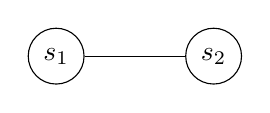
\begin{tikzpicture}[every node/.style={circle,draw}]
\node (1) at (0,0) {$s_1$}; \node (2) at (2,0) {$s_2$}; \path (1) edge (2);
\end{tikzpicture}
\caption{Two-spin Ising graph for the MH toy example.}
\end{figure}
\end{example}


\paragraph{Gibbs sampling.}
Gibbs sampling is a special case of the Metropolis--Hastings algorithm in which the proposal distribution is chosen to be the exact conditional distribution of one variable given the others. Because such proposals are always accepted, Gibbs sampling eliminates the need for an explicit acceptance step, making it one of the simplest and most widely used MCMC algorithms \citep{geman_stochastic_1984}. The method proceeds by iteratively resampling each variable $x_i$ from its conditional distribution $p(x_i \mid x_{-i})$, where $x_{-i}$ denotes all variables except $x_i$. By the Markov property of MRFs, this conditional depends only on the neighbors $N(i)$ of $i$ in the graph, which greatly reduces the computational cost in sparse models.

Gibbs sampling has several attractive features. It is easy to implement whenever conditionals are available in closed form, and in models with local interactions it naturally exploits the structure of the graph. In pairwise Markov random fields such as the Ising model, the conditional distribution of a single spin depends only on the sum of the neighboring spins, yielding a simple logistic form. Moreover, since Gibbs sampling updates one variable at a time, it can be seen as a stochastic analogue of coordinate descent in the energy landscape. These properties have made Gibbs sampling a standard inference method in fields ranging from image analysis and Bayesian networks to the training of Boltzmann machines.

Nevertheless, standard Gibbs sampling can suffer from poor mixing in high-dimensional or multimodal distributions, where single-variable updates are insufficient to traverse energy barriers efficiently. To mitigate this, several variants have been developed. \emph{Block Gibbs sampling} updates groups of variables jointly rather than individually, reducing correlations between successive samples and improving convergence in strongly coupled systems \citep{liu_monte_2001}. Another widely used extension is \emph{parallel tempering} (also known as replica exchange MCMC), where multiple chains are run at different temperatures and periodically exchange states. This approach helps overcome slow mixing in rugged energy landscapes by allowing high-temperature chains to explore broadly and low-temperature chains to refine local structure \citep{geyer_markov_1991}. These and related techniques demonstrate the adaptability of Gibbs sampling to challenging inference tasks.

A more detailed analysis of such limitations and variants, especially in the discrete and combinatorial settings central to this thesis, will be deferred to later chapters once combinatorial optimization problems have been formally introduced.

\begin{algorithm}[htbp]
\caption{Gibbs sampling}
\KwData{Factorization $\{\psi_c\}$; schedule over variables}
\KwResult{Samples $\{x_t\}$}
Initialize $x$; \For{$t=0$ {\bf to} $T-1$}{\For{each variable $i$ (in random or fixed order)}{Sample $x_i \sim p(x_i \mid x_{N(i)}) \propto \prod_{c\ni i}\psi_c(x_c).$}}
\end{algorithm}

\begin{example}{\hrule\vspace{.2em}Gibbs on a $2\times 2$ Ising grid\vspace{.2em}\hrule}
Consider four binary spins $\{s_1,s_2,s_3,s_4\}$ arranged in a square with pairwise potential $\psi(s_i,s_j)=\exp(J s_is_j)$. By the Markov property, the conditional distribution of $s_1$ given its neighbors depends only on $s_2$ and $s_3$, and is given by
\[
p(s_1=+1 \mid s_2,s_3) \propto \exp\!\big(J(s_2+s_3)\big).
\]
The Gibbs sampler cycles through the four spins, repeatedly resampling each from its conditional. Over time, the sequence of states produced by this process approximates the Boltzmann distribution of the grid.


\begin{figure}[htbp]\centering
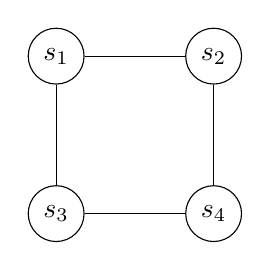
\begin{tikzpicture}[every node/.style={circle,draw}]
\node (1) at (0,0) {$s_1$}; \node (2) at (2,0) {$s_2$};
\node (3) at (0,-2) {$s_3$}; \node (4) at (2,-2) {$s_4$};
\path (1) edge (2); \path (1) edge (3); \path (2) edge (4); \path (3) edge (4);
\end{tikzpicture}\caption{$2\times 2$ Ising grid for Gibbs sampling.}\end{figure}
\end{example}


\paragraph{Importance sampling (IS).}
Classical importance sampling is a general Monte Carlo technique for estimating expectations under a complex distribution $p$ by drawing samples from a simpler proposal distribution $q$ and reweighting them. Given $x^{(i)}\sim q$, the self-normalized estimator of $\mathbb{E}_p[f(X)]$ is
\begin{equation}
\widehat{\mathbb{E}}_p[f]=\frac{\sum_{i=1}^N w^{(i)} f(x^{(i)})}{\sum_{i=1}^N w^{(i)}},\qquad w^{(i)}=\frac{p(x^{(i)})}{q(x^{(i)})}.
\end{equation}
The efficiency of IS depends critically on the quality of the proposal $q$: if $q$ does not overlap well with $p$, the variance of the estimator explodes and the effective sample size $\mathrm{ESS}=\tfrac{(\sum_i w^{(i)})^2}{\sum_i (w^{(i)})^2}$ becomes very small. For high-dimensional discrete Boltzmann distributions, constructing such good proposals is generally infeasible, which is why IS is rarely used directly in this context.

It is worth noting, however, that in the MRF literature the term ``importance sampling'' has sometimes been applied to a different family of algorithms designed for inference with evidence. In these settings, some variables are clamped to observed values and we wish to sample from the conditional distribution of the remaining free variables. One approximate strategy is to sample variables sequentially, fixing each to a value and adjusting the potentials of the factors involving it before proceeding to the next variable. This procedure can be interpreted as a form of \emph{sequential importance sampling}, where variables are generated one at a time and the distribution is updated accordingly. While the name is the same, it is important to distinguish this specialized conditional sampling from the classical IS estimator described above.

Finally, a number of extensions of IS have been proposed to make it more practical in complex models. \emph{Annealed importance sampling (AIS)} \citep{neal_annealed_1998} gradually transforms an easy-to-sample distribution into the target by introducing a sequence of intermediate distributions, while \emph{sequential importance sampling (SIS)} and related particle filtering methods \citep{doucet_sequential_2001} adapt the proposal distribution step by step as variables are sampled. These approaches are widely used in Bayesian inference and for estimating partition functions of energy-based models. Although they remain challenging to apply efficiently to large-scale combinatorial structures, they provide important conceptual links between IS and the more flexible MCMC strategies introduced earlier.

\begin{example}{\hrule\vspace{.2em}Sequential IS heuristic for MIS\vspace{.2em}\hrule}
For the Maximum Independent Set problem on a graph $G$, one may define a sequential proposal that samples vertices in some order, with probabilities biased by degree. Each time a vertex is chosen, its neighbors are excluded from further consideration, and the process continues until no more vertices can be added. The resulting independent set $S$ is feasible by construction, but biased by the sampling order. Importance weights can, in principle, be assigned to correct this bias, yielding an instance of sequential importance sampling adapted to a combinatorial constraint.
\end{example}

\paragraph{Sequential Importance Sampling (SIS).}  
In this thesis, whenever we refer to \emph{Importance Sampling} for Markov Random Fields, we specifically mean the \emph{Sequential Importance Sampling} (SIS) algorithm. Unlike the classical IS estimator that draws i.i.d.\ samples from a static proposal distribution, SIS generates samples sequentially by progressively fixing variables and adjusting the factor potentials of the remaining subproblem. This is particularly well-suited for discrete graphical models and combinatorial problems, since feasibility constraints can be enforced at each step of the sequence.  

Formally, let $X=(X_1,\dots,X_n)$ be the set of variables. SIS constructs a sequence of intermediate target distributions $p^{(1)},\dots,p^{(n)}$, where at step $t$ a variable $X_t$ is sampled conditioned on previously fixed variables. Importance weights are updated multiplicatively, correcting for proposal bias.  

\begin{algorithm}[htbp]
\caption{Sequential Importance Sampling for MRFs}
\KwData{Factor graph $H=(V,F,E)$ with potentials $\{\psi_f\}$}
\KwResult{Weighted samples $\{(x^{(i)}, w^{(i)})\}_{i=1}^N$}
\For{$i=1$ {\bf to} $N$}{
  Initialize weight $w^{(i)}=1$\;
  \For{$t=1$ {\bf to} $n$}{
    Sample $x_t^{(i)} \sim q_t(\cdot \mid x_{1:t-1}^{(i)})$\;
    Update weight 
    $w^{(i)} \gets w^{(i)} \cdot \frac{p(x_{1:t}^{(i)})}{q_t(x_t^{(i)} \mid x_{1:t-1}^{(i)})}$\;
  }
}
Normalize weights: $\tilde{w}^{(i)} = w^{(i)}/\sum_j w^{(j)}$\;
\end{algorithm}

SIS produces a weighted empirical approximation of the MRF distribution,
\[
\hat{p}(x) = \sum_{i=1}^N \tilde{w}^{(i)} \, \delta_{x^{(i)}}(x),
\]
that can be used to estimate marginals, guide greedy decoding, or construct approximate solutions. While SIS mitigates some of the difficulties of naive IS in high-dimensional discrete spaces, it remains sensitive to proposal design and can suffer from weight degeneracy, particularly when the sampling order is poorly chosen or dependencies between variables are strong \citep{doucet_sequential_2001, cappe_inference_2005}.



\subsection{Graphical models}
Graphical models provide a unifying framework for representing complex multivariate probability distributions using graphs. The central idea is that statistical dependencies among random variables can be expressed in terms of the edges of a graph, so that the global distribution factorizes into a product of local functions associated with the graph structure \citep{wainwright_graphical_2007}. This factorization makes explicit which variables interact directly and which are conditionally independent given others, allowing compact specification of high-dimensional distributions and enabling scalable inference algorithms.

Two broad families of graphical models are commonly distinguished. In \emph{directed graphical models} (also known as Bayesian networks), edges represent directed dependencies and the joint distribution factorizes into conditional probabilities along these edges. These models are well suited for encoding causal relationships and are widely used in probabilistic reasoning and learning. In \emph{undirected graphical models}, also called Markov Random Fields (MRFs) or Gibbs random fields, edges represent undirected interactions, and the joint distribution factorizes according to cliques of the graph. This representation is particularly natural for energy-based formulations, where probabilities are defined in terms of an energy function and the Boltzmann distribution. 

In this thesis, we focus exclusively on undirected graphical models, since they provide the appropriate language for expressing combinatorial optimization problems in terms of energy minimization. MRFs allow constraints and objective functions to be encoded locally through potentials on nodes and edges, while factor graphs offer a bipartite representation that makes the structure of inference algorithms such as belief propagation more transparent. These models connect directly to the Boltzmann distributions introduced in the previous section and form the foundation for the study of approximate inference methods. The following subsections introduce Markov Random Fields and factor graphs in more detail, before turning to inference procedures, with particular emphasis on message passing algorithms.


\subsubsection{Markov random fields}
Markov Random Fields (MRFs), also known as undirected graphical models or Gibbs random fields, provide a powerful way to represent structured probability distributions in terms of local interactions. Formally, let $G=(V,E)$ be an undirected graph, where each vertex $v \in V$ corresponds to a random variable $X_v$, and let $X=(X_v)_{v\in V}$ denote the collection of variables. The graph encodes conditional independence assumptions stated in the following definition :

\begin{definition}[Markov Property]
\label{def:markov_property}
Let $G=(V,E)$ be an undirected graph and $X=(X_v)_{v\in V}$ a collection of random variables with domain $\mathcal{X}=\otimes_{v\in V} \mathcal{X}_v$. A distribution $p(\cdot)$ of $X$ is said to have the \emph{Markov property} with respect to graph $G$ if the following holds : 

$$X_i \perp\!\!\!\perp X_{V\setminus(\{i\}\cup N(i))}\;\mid\;X_{N(i)}, $$

meaning that each variable is independent of all others given its neighbors $N(i)$ in the graph.

\end{definition}

The Markov property reflects the intuitive idea that in an MRF, dependence is mediated only through local connections. The family of distributions that have the Markov property with respect to a graph $G$ is called an MRF.

\begin{definition}[Graph separation]
Let $G=(V,E)$ be an undirected graph, and let $A,B,C \subseteq V$ be disjoint sets of nodes. We say that $C$ \emph{separates} $A$ and $B$ in $G$ if every path from a node in $A$ to a node in $B$ passes through at least one node in $C$.
\end{definition}

\begin{proposition}[Global Markov property]
Let $p(\cdot)$ be a distribution that is Markov with respect to $G$. For any disjoint sets $A,B,C \subseteq V$, if $C$ separates $A$ and $B$ in $G$, then
\[
X_A \perp\!\!\!\perp X_B \mid X_C.
\]
\end{proposition}

This property provides a direct graphical interpretation of conditional independence: dependencies between variables can be understood by inspecting paths in the graph. Conditioning on a set of variables $C$ effectively blocks all paths passing through $C$, rendering variables in $A$ and $B$ independent.

\begin{definition}[Markov Random Field]
\label{def:markov_random_field}
Given an undirected graph $G=(V,E)$ and a collection of corresponding random variables $X=(X_v)_{v\in V}$. A Markov Random Field with respect to $G$ is the family of probability distributions on $X$ that satisfy the Markov property ~\ref{def:markov_property} with respect to $G$.
\end{definition}

The Hammersley–Clifford theorem \cite{besag_spatial_1974,grimmett_theorem_1973,grimmett_disorder_1990} establishes the equivalence between the Markov property and a factorization over the cliques of the graph.

\begin{theorem}[Hammersley-Clifford theorem]
\label{thm:hammersley_clifford_theorem}
Any strictly positive distribution $p(\cdot)$ that respects the Markov property with respect to an undirected graph $G=(V,E)$ can be written in factorized form over the cliques $\mathcal{C}(G)$ of the graph:
\begin{equation}
p(x)=\frac{1}{Z}\prod_{c\in\mathcal{C}(G)}\psi_c(x_c),
\end{equation}
where $\psi_c(x_c)\geq 0$ is a potential function defined on clique $c$, and $Z=\sum_{x\in\mathcal{X}} \prod_{c\in\mathcal{C}(G)}\psi_c(x_c)$ ensures normalization and is called the \emph{partition function}. Conversely, any strictly positive distribution that factorizes over the cliques of $G$ satisfies the Markov property with respect to $G$.
\end{theorem}

Potentials can be interpreted as local energy contributions by defining $E_c(x_c) = -\log \psi_c(x_c)$. Taking logarithms, the distribution can always be written in Gibbs form:
\begin{equation}
p(x)=\frac{1}{Z}\exp\!\Big(\sum_{c\in\mathcal{C}(G)} \log \psi_c(x_c)\Big).
\end{equation}

A particularly important class of distributions is given by the exponential family, which provides a natural parametrization of such models.

\begin{definition}[Exponential family]
\label{def:exponential_family}
A family of probability distributions $\{p(x;\theta)\}_{\theta \in \Theta}$ on $\mathcal{X}$ is said to belong to the exponential family if it can be written in the form
\begin{equation}
p(x;\theta) = \frac{1}{Z(\theta)} \exp\!\big( \langle \theta, \phi(x) \rangle \big),
\end{equation}
where $\phi(x)$ is a vector of sufficient statistics (feature functions), $\theta$ is a vector of parameters, and $Z(\theta)$ is the partition function ensuring normalization.
\end{definition}

In the context of MRFs, this parametrization arises naturally when the clique potentials are expressed as
\[
\psi_c(x_c;\theta_c) = \exp\big(\theta_c^\top \phi_c(x_c)\big).
\]
In this case, the resulting distribution takes the exponential-family form
\begin{equation}
p(x;\theta)=\frac{1}{Z(\theta)}\exp\!\Big(\sum_{c\in\mathcal{C}(G)} \theta_c^\top \phi_c(x_c)\Big),
\end{equation}
where the global feature vector $\phi(x)$ decomposes as a sum of local clique features and $\theta = (\theta_c)_{c\in \mathcal{C}(G)}$ are the parameters of the distribution. In this formulation, the graph structure determines the decomposition of the sufficient statistics, while the parameters control the strength of local interactions.

Table~\ref{tab:exp_family_examples} illustrates how different choices of sufficient statistics and parameters recover well-known distributions. In particular, pairwise and higher-order MRFs correspond to exponential-family distributions whose sufficient statistics decompose over the structure of the graph. This decomposition will be central in our approach, where the parameters associated with these features are predicted by a neural network. 
\begin{table}[htbp]
\centering
\begin{tabular}{lccc}
\toprule
\textbf{Distribution} & \textbf{Support} & $\boldsymbol{\phi(x)}$ & \textbf{Parameters $\boldsymbol{\theta}$} \\
\midrule

Bernoulli & $x \in \{0,1\}$ 
& $x$ 
& $\log\!\left(\frac{p}{1-p}\right)$ \\

Categorical & $x \in \{1,\dots,K\}$ 
& $\mathbf{1}[x = k]$ 
& $\log \pi_k$ \\

Multinomial & $x \in \mathbb{N}^K$ 
& $x_k$ 
& $\log \pi_k$ \\

Gaussian (1D) & $x \in \mathbb{R}$ 
& $(x,\; x^2)$ 
& $(\mu/\sigma^2,\; -\tfrac{1}{2\sigma^2})$ \\

Multivariate Gaussian & $x \in \mathbb{R}^n$ 
& $(x,\; xx^\top)$ 
& $(\Sigma^{-1}\mu,\; -\tfrac{1}{2}\Sigma^{-1})$ \\

Poisson & $x \in \mathbb{N}$ 
& $x$ 
& $\log \lambda$ \\

Ising model & $x \in \{-1,1\}^n$ 
& $(x_i,\; x_i x_j)$ 
& $(h_i,\; J_{ij})$ \\

Pairwise MRF & $x \in \mathcal{X}^n$ 
& $(\phi_i(x_i),\; \phi_{ij}(x_i,x_j))$ 
& $(\theta_i,\; \theta_{ij})$ \\

\bottomrule
\end{tabular}
\caption{Examples of exponential-family distributions obtained from different sufficient statistics and parameters.}
\label{tab:exp_family_examples}
\end{table}



The expressiveness of MRFs makes them well suited for modeling structured domains such as images, spatial data, and graphs, where local interactions govern global behavior. However, inference in general MRFs is computationally challenging. Computing the partition function $Z$ requires summing over all possible configurations of $X$, which grows exponentially with the number of variables. Similarly, computing marginal probabilities or the most likely configuration (MAP inference) is tractable only for graphs with very limited structure (e.g., trees or graphs of small treewidth). In fact, exact inference in MRFs is \#P-hard in general \citep{chandrasekaran_complexity_2008}, which motivates the development of approximate inference algorithms such as belief propagation, variational methods, and sampling techniques. These will be introduced in subsequent sections.

In the context of this thesis, MRFs serve as the core formalism for linking energy-based models to combinatorial optimization. By designing potential functions $\psi_c$ that encode local constraints and objectives, many optimization problems can be expressed as inference tasks in an MRF, with low-energy states corresponding to high-quality solutions. In this work, we consider parametrized MRF distributions, where the graph structure is fixed and the potentials are learned from data.


\subsubsection{Factor graphs}
Factor graphs provide an alternative representation of graphical models that makes the factorization structure of the distribution explicit. Formally, a factor graph is a bipartite graph $H=(V \cup \FACTORSET,E_H)$ consisting of variable nodes $\VCGV$ corresponding to random variables $\{\XRAV_i : i\in \VCGV \}$ and factor nodes $\FACTORSET$ corresponding to potential functions $\{\psi_{\FACTOR} : \FACTOR\in \FACTORSET\}$. An edge $(i,\FACTOR)\in E_H$ indicates that variable $\XRAV_i$ participates in factor $\psi_{\FACTOR}(x_{\FACTOR})$. The joint distribution over all variables then factorizes as
\[
p(x) = \frac{1}{Z}\prod_{\FACTOR\in \FACTORSET}\psi_{\FACTOR}(x_{\FACTOR}).
\]
This representation generalizes both directed and undirected graphical models by explicitly distinguishing between variables and the factors that constrain them \citep{wainwright_graphical_2007}.

One of the key advantages of factor graphs is that they make message-passing algorithms such as the sum--product and max--product algorithms particularly transparent. Messages are naturally passed along edges between variables and factors, and the bipartite structure enforces a clean separation between the two types of updates. This is especially useful in large-scale problems where inference relies on local computations that can be distributed across the graph.

Factor graphs also provide a flexible modeling tool for combinatorial optimization. Local constraints, such as adjacency restrictions in independent set problems or coverage requirements in vertex cover, can be encoded as factor nodes that enforce specific interactions among variables. This modularity allows complex global objectives to be built up from simple local potentials, aligning closely with the energy-based modeling perspective introduced earlier.

\begin{example}{\hrule\vspace{.2em}Factor-graph view of a chain\vspace{.2em}\hrule}
\vspace{1em}
%\todo{figure missing} 
Consider a simple chain $X_1$--$X_2$--$X_3$ with pairwise factors $\psi_{12}(x_1,x_2)$ and $\psi_{23}(x_2,x_3)$ as well as unary factors $\phi_i(x_i)$. The corresponding factor graph has variable nodes $\{1,2,3\}$ and factor nodes $\{\psi_{12},\psi_{23},\phi_1,\phi_2,\phi_3\}$, with edges connecting each factor to the variables it depends on. This bipartite structure highlights how the distribution factorizes and directly supports the mechanics of sum--product message passing.

\begin{figure}[htbp]\centering
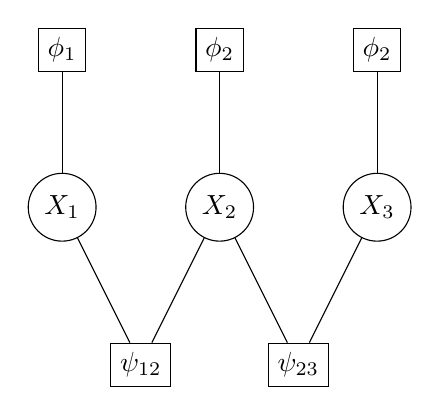
\begin{tikzpicture}[var/.style={circle,draw},factor/.style={rectangle,draw}]
\node[var] (x1) at (0,0) {$X_1$}; 
\node[var] (x2) at (2,0) {$X_2$};
\node[var] (x3) at (4,0) {$X_3$};
\node[factor] (u1) at (0,2) {$\phi_1$};
\node[factor] (u2) at (2,2) {$\phi_2$};
\node[factor] (u3) at (4,2) {$\phi_2$};
\node[factor] (p12) at (1,-2) {$\psi_{12}$};
\node[factor] (p23) at (3,-2) {$\psi_{23}$};
\path (x1) edge (u1); \path (x2) edge (u2); \path (x3) edge (u3);
\path (x1) edge (p12); \path (x2) edge (p12);
\path (x2) edge (p23); \path (x3) edge (p23);
\end{tikzpicture}\caption{Simple factor graph with $3$ variables, unary and pairwise factors.}
\end{figure}

\end{example}

In summary, factor graphs not only unify the representation of directed and undirected models but also provide the natural stage on which message-passing inference algorithms operate. For this reason, they will serve as a central tool in later chapters when we study inference in Markov random fields and its application to combinatorial optimization problems.

\paragraph{Canonical over-complete representation.}
For discrete graphical models, an equivalent but often more convenient parameterization is obtained through the canonical over-complete representation. Rather than associating features with a minimal set of sufficient statistics, one introduces indicator functions for every local assignment of each variable and factor. For a factor graph with variables $X_i \in \mathcal{X}_i$ and factors $F \in \mathcal{F}$, the unary sufficient statistics are
\begin{equation}
\phi_{i,y}(x)=\mathbbm{1}\{x_i=y\}, \qquad y\in\mathcal{X}_i,
\end{equation}
while the factor sufficient statistics are
\begin{equation}
\phi_{\FACTOR,y_{\FACTOR}}(\XVEC)=\mathbbm{1}\{\XFACT=y_{\FACTOR}\}, \qquad y_{\FACTOR}\in\mathcal{X}_{\FACTOR} .
\end{equation}
The corresponding exponential-family distribution can then be written as
\begin{equation}
p_{\EPARAM}(\XVEC)
=
\exp\left(
\sum_{i\in \VCGV}\sum_{y\in\mathcal{X}_i}\EPARAM_{i,y}\phi_{i,y}(\XVEC)
+
\sum_{\FACTOR\in\FACTORSET}\sum_{y_{\FACTOR}\in\mathcal{X}_{\FACTOR}}
\theta_{\FACTOR,y_{\FACTOR}}\phi_{\FACTOR,y_{\FACTOR}}(\XVEC)
-
A(\theta)
\right).
\end{equation}
This representation is called over-complete because the indicator statistics are linearly dependent: for each variable or factor, exactly one local configuration is active, so the associated indicators sum to one. Consequently, the natural parameters are not identifiable without additional constraints or gauge choices. Nevertheless, the over-complete form is particularly useful for graphical models because it aligns directly with local potentials, marginal inference, and variational relaxations. In this parameterization, learning can still be interpreted as moment matching, but the moments now correspond to unary and factor marginals. Approximate inference algorithms such as belief propagation therefore naturally operate on these quantities, returning beliefs $\mu_i(\XVEC_i)$ and $\mu_{\FACTOR}(x_{\FACTOR})$ that approximate the marginal expectations of the corresponding indicator sufficient statistics \cite{wainwright_graphical_2007}. When we refer to \emph{over-complete parameters}, we mean natural parameters whose entries are indexed by this over-complete set of indicator sufficient statistics. Thus, over-completeness is formally a property of the sufficient-statistic representation, not of the parameters themselves; the parameters are called over-complete only as shorthand for being compatible with that representation.


\subsection{Inference and Belief Propagation}
In graphical models, \emph{inference} refers to the set of tasks through which one extracts useful probabilistic information from a factorized distribution. The most common forms are: computing marginal distributions of individual variables or subsets of variables, estimating conditional probabilities given evidence, evaluating the partition function, and solving for the maximum a posteriori (MAP) configuration. Each of these problems is central to applications of Markov Random Fields: marginals provide uncertainty estimates, the partition function controls normalization and likelihood evaluation, and MAP inference directly corresponds to combinatorial optimization by identifying the lowest-energy configuration.

Exact inference is only tractable for models with restricted structure, such as trees or graphs with small treewidth. For general graphs, marginal inference and partition function computation are \#P-hard, while MAP inference is NP-hard \citep{chandrasekaran_complexity_2008,schrijver_combinatorial_2003}. As a result, research has focused on approximate inference algorithms. Two major families dominate: sampling-based approaches such as Markov Chain Monte Carlo \citep{geman_stochastic_1984} and deterministic algorithms based on variational approximations \citep{wainwright_graphical_2007}. Among the latter, message-passing algorithms are particularly appealing because they exploit the structure of factor graphs to perform distributed local computations.

\emph{Belief Propagation} (BP) is the canonical message-passing algorithm for inference in factor graphs. In its sum--product form, BP computes approximate marginal distributions by iteratively exchanging messages between variable nodes and factor nodes. In its max--product form, the algorithm approximates MAP inference by replacing summations with maximizations. On tree-structured graphs, both algorithms are exact and run in time linear in the number of edges, making BP highly efficient in this setting. On graphs with cycles, the same iterative procedure can still be applied; in this case it is known as \emph{loopy BP}. Although not guaranteed to converge, loopy BP often provides remarkably accurate approximations in practice and has been shown to correspond to stationary points of the Bethe free energy \citep{yedidia_understanding_2003}.

For this thesis, inference plays a dual role. On the one hand, it is the computational mechanism through which probabilistic quantities and approximate solutions to combinatorial problems are obtained. On the other hand, because many inference algorithms such as BP can be expressed as differentiable computational graphs, they can be embedded into end-to-end trainable architectures. This differentiability enables the backpropagation of gradients through the inference process, allowing parameters of neural networks or energy functions to be learned directly by gradient descent. This approach stands in contrast to alternative methods such as MAP-perturbation techniques \citep{tarlow_randomized_2012,papandreou_perturb-and-map_2011,nowozin_perturb-and-map_2014}, which approximate gradients indirectly via sampling perturbed MAP solutions. By leveraging differentiable inference, our work integrates the structure and interpretability of MRFs with the flexibility of modern deep learning, setting the stage for the contributions developed in later chapters.


\subsubsection{Sum--product BP (marginals)}
The sum--product algorithm, also known as Belief Propagation (BP), is a message-passing procedure for computing marginal distributions in factor graphs. Its central idea is that local computations on the bipartite structure of the factor graph can be combined to yield global information about the distribution. On tree-structured graphs, the algorithm is exact and runs in time linear in the number of edges; on graphs with cycles it becomes an approximation, known as \emph{loopy BP}, which nevertheless performs surprisingly well in many applications \citep{yedidia_understanding_2003,kschischang_factor_2001}.

Formally, let $H=(V\cup F,E_H)$ be a factor graph. Messages are passed iteratively along edges from variables to factors and from factors to variables:
\begin{align}
m_{i\rightarrow f}(x_i) &= \prod_{g\in N(i)\setminus\{f\}} m_{g\rightarrow i}(x_i),\\
m_{f\rightarrow i}(x_i) &= \sum_{x_{f\setminus i}} \psi_f(x_f)\prod_{j\in f\setminus i} m_{j\rightarrow f}(x_j).
\end{align}
Variable-to-factor messages represent the belief of a variable node about its state based on all other neighboring factors, while factor-to-variable messages aggregate information from neighboring variables mediated by the factor potential. Once messages have converged (or after a fixed number of iterations), approximate beliefs are computed as
\[
b_i(x_i)\propto \prod_{f\in N(i)} m_{f\rightarrow i}(x_i), \qquad 
b_f(x_f)\propto \psi_f(x_f)\prod_{i\in f} m_{i\rightarrow f}(x_i).
\]
These beliefs approximate marginal distributions for nodes and factors. On trees, they coincide exactly with the true marginals.

\begin{algorithm}[htbp]
\caption{Sum--product Belief Propagation}
\KwData{Factor graph $H=(V\cup F,E_H)$, messages $\{m\}$}
\KwResult{Approx.\ beliefs $\{b_i,b_f\}$}
Initialize all messages (e.g., uniformly);\;
\Repeat{convergence or max-iter}{
\ForEach{$(i,f)\in E_H$}{
Update $m_{i\to f}$ and $m_{f\to i}$ according to the update equations.}}
Compute beliefs $b_i, b_f$ from messages.\;
\end{algorithm}

The sum--product algorithm can be interpreted from multiple perspectives. It arises naturally as dynamic programming on trees, as variational optimization of the Bethe free energy \citep{yedidia_understanding_2003}, and as exact marginalization in factor graphs of bounded treewidth. In loopy graphs, fixed points of the message updates correspond to stationary points of the Bethe free energy, providing a variational justification for its use. From a computational viewpoint, the algorithm distributes the intractable global inference task into many local updates, each involving only small subsets of variables. This locality makes BP highly scalable and parallelizable, which explains its widespread use in areas such as error-correcting codes, computer vision, and structured prediction in machine learning.

In the context of this thesis, the sum--product algorithm is important not only as a classical inference method but also because its iterative updates are differentiable operations. This property allows BP to be unrolled and integrated into neural architectures, enabling backpropagation of gradients through the inference process. By embedding differentiable BP into training, we can jointly optimize parameters of energy functions and neural networks while respecting the graphical structure of the problem.


\paragraph{Max--product BP (MAP)}
Replacing $\sum$ by $\max$ (and products by sums in log domain) yields max--product; on trees it recovers dynamic programming for MAP. On loopy graphs, convergence is not guaranteed; convex variants such as tree-reweighted message passing (TRW/ TRW-S) provide bounds and convergence guarantees for specific energies \citep{kolmogorov_convergent_2006}.


\subsubsection{When and why does BP work?}
Belief Propagation is exact on trees, but on graphs with cycles its behavior is more subtle. Empirically, loopy BP has been found to give high-quality approximations in many applications, from error-correcting codes to computer vision, even when theoretical guarantees are lacking. Understanding the regimes in which BP provides correct results has therefore been an important line of research.

Beyond trees, BP is known to provably solve certain classes of combinatorial optimization problems. For example, it exactly recovers maximum-weight matchings and $b$-matchings under appropriate conditions \citep{bayati_maximum_2005, huang_loopy_2007, bayati_belief_2011, shin_graphical_2013}, and can solve instances of min-cost flow \citep{gamarnik_belief_2012}. These results demonstrate that, despite its heuristic nature in loopy graphs, BP can coincide with exact combinatorial algorithms in structured settings. On the practical side, distributed and parallel implementations \citep{gonzalez_parallel_2010, ma_task_2012} allow BP to scale to very large graphs, making it attractive in network and graph mining applications.

It is also worth clarifying terminology: the \emph{sum--product} algorithm is used for computing marginals, while the \emph{max--product} algorithm is its counterpart for MAP inference. The latter is often implemented in log-space, in which case products of probabilities become sums of log-probabilities, yielding the so-called \emph{max--sum} algorithm. The two names thus refer to the same underlying procedure, with max--sum being a numerically more stable implementation. This distinction helps to situate BP within the broader family of dynamic programming methods such as the Viterbi algorithm, which also operates in the max--sum (log-space) domain.

Despite these successes, BP also has well-documented limitations. On loopy graphs, it may fail to converge or converge to poor fixed points. Techniques such as damping, residual scheduling, and convex free-energy approximations can mitigate these issues but do not eliminate them entirely \citep{yedidia_understanding_2003, kolmogorov_convergent_2006}. Furthermore, when factors involve many variables or when variables have large alphabets, the size of messages becomes prohibitive. In such cases, structured factors and low-rank approximations can be used in practice to reduce complexity \citep{wainwright_graphical_2007}.


\subsubsection{Learning-augmented Belief Propagation}
While classical BP is purely algorithmic and determined by the graphical model structure and its potentials, recent research has explored how learning can be used to augment or modify the BP procedure itself. The motivation is twofold: first, to overcome some of the limitations of standard BP, such as poor convergence or inaccurate marginals on loopy graphs; and second, to integrate inference more tightly with modern machine learning pipelines where parameters are trained end-to-end.

Learning can intervene at several levels of the BP algorithm. One approach is to make the \emph{messages} themselves parametric and learnable, so that instead of strictly following the sum--product or max--product updates, neural networks predict or reweight the messages passed along edges. This idea underlies neural message-passing architectures that generalize BP by embedding richer computations within each update \citep{satorras_neural_2021}. A second approach is to learn the \emph{message schedule}, i.e., the order and frequency with which messages are updated. By training update schedules on data, convergence speed and accuracy can often be improved relative to fixed synchronous or asynchronous schemes. A third line of work uses learning to adapt the \emph{potentials} of the graphical model itself, either by parameterizing them with neural networks or by amortizing inference across many instances of a problem class \citep{wiseman_amortized_2019}.

These developments fall under the broader paradigm of \emph{learning to infer}, where inference algorithms are not treated as fixed black boxes but as differentiable computational graphs whose parameters can be optimized from data. Differentiable BP variants allow gradients to be propagated through the inference process, enabling neural networks to be trained with feedback that depends on approximate marginals or MAP configurations. This sets them apart from sampling-based gradient estimators or MAP-perturbation methods \citep{tarlow_randomized_2012,nowozin_perturb-and-map_2014}, which do not permit exact backpropagation.



\begin{figure}[htbp]
\centering
\begin{tikzpicture}[node distance=2cm, every node/.style={font=\small}]
  % Variable nodes
  \node[circle,draw,minimum size=0.8cm] (x1) {$x_1$};
  \node[circle,draw,minimum size=0.8cm, right of=x1] (x2) {$x_2$};
  \node[circle,draw,minimum size=0.8cm, right of=x2] (x3) {$x_3$};
  % Factor nodes
  \node[rectangle,draw,minimum width=0.9cm,minimum height=0.6cm,below of=x1,node distance=1.5cm] (f1) {$\psi_1$};
  \node[rectangle,draw,minimum width=0.9cm,minimum height=0.6cm,below of=x2,node distance=1.5cm] (f2) {$\psi_{12}$};
  \node[rectangle,draw,minimum width=0.9cm,minimum height=0.6cm,below of=x3,node distance=1.5cm] (f3) {$\psi_2$};
  % Edges
  \draw (x1) -- (f1);
  \draw (x1) -- (f2);
  \draw (x2) -- (f2);
  \draw (x2) -- (f3);
  \draw (x3) -- (f3);
  % Neural annotation
  \node[below=0.8cm of f2,font=\footnotesize,align=center] (nn) {Neural module \\ adapting messages};
  \draw[->,dashed] (nn.north) -- (f2.south);
\end{tikzpicture}
\caption{Schematic illustration of learning-augmented Belief Propagation. 
Classical messages (solid edges) are complemented by neural modules (dashed arrow) that reweight or adapt updates.}
\end{figure}

In this thesis, learning-augmented BP will play a central role. We will exploit the differentiability of message passing to integrate it directly into our models for combinatorial optimization. By combining the structure and interpretability of BP with the flexibility of neural networks, we aim to design inference mechanisms that are both expressive and trainable, bridging the gap between classical graphical model inference and modern deep learning approaches.



\begin{example}{\hrule\vspace{.2em}BP on a chain (exact)\vspace{.2em}\hrule}
For a chain $X_1$--$X_2$--$X_3$ with unary and pairwise factors $\{\phi_1,\phi_2,\phi_3,\psi_{12}, \psi_{23}\}$. During belief propagation, messages are iteratively exchanged along the edges between variables and factors. Each variable sends a \emph{variable-to-factor} message $q_{i \to F}$ that summarizes its current belief based on all other connected factors, while each factor sends a \emph{factor-to-variable} message $r_{F \to i}$ encoding the compatibility of variable states given its neighboring messages. After several iterations, these messages converge toward consistent marginal or MAP estimates for the variables. This simple three-variable example illustrates the bidirectional flow of information that underlies both sum-product and max-product belief propagation.


\begin{figure}[htbp]\centering
\begin{tikzpicture}[
  >=Latex,
  var/.style={circle,draw,minimum size=18pt,inner sep=1pt},
  factor/.style={rectangle,draw,rounded corners=0pt,minimum width=16pt,minimum height=12pt,inner sep=2pt},
  graphedge/.style={line width=0.5pt},
  msgVF/.style={->,thick,blue!70,shorten <=2pt,shorten >=2pt},
  msgFV/.style={->,thick,red!70,shorten <=2pt,shorten >=2pt},
  msglabel/.style={font=\scriptsize,fill=white,inner sep=1pt}
]

% --- Nodes
\node[var]    (x1) at (0,0)   {$X_1$}; 
\node[var]    (x2) at (4,0)   {$X_2$};
\node[var]    (x3) at (8,0)   {$X_3$};
\node[factor] (u1) at (0,2)   {$\FACTOR_1$};
\node[factor] (u2) at (4,2)   {$\FACTOR_2$};
\node[factor] (u3) at (8,2)   {$\FACTOR_2$}; % keep as provided
\node[factor] (p12) at (2,-2) {$\FACTOR_{12}$};
\node[factor] (p23) at (6,-2) {$\FACTOR_{23}$};

% --- Undirected factor-graph edges
\path[graphedge] (x1) -- (u1);
\path[graphedge] (x2) -- (u2);
\path[graphedge] (x3) -- (u3);
\path[graphedge] (x1) -- (p12);
\path[graphedge] (x2) -- (p12);
\path[graphedge] (x2) -- (p23);
\path[graphedge] (x3) -- (p23);

% --- Message arrows (one iteration t)
% Unary factors
\draw[msgVF,bend left=28] (x1) to node[msglabel,pos=0.5] {$m_{1\rightarrow \FACTOR_1}$} (u1);
\draw[msgFV,bend left=28] (u1) to node[msglabel,pos=0.5] {$m_{\FACTOR_1\rightarrow 1}$} (x1);

\draw[msgVF,bend left=28] (x2) to node[msglabel,pos=0.5] {$m_{2\rightarrow \FACTOR_2}$} (u2);
\draw[msgFV,bend left=28] (u2) to node[msglabel,pos=0.5] {$m_{\FACTOR_2\rightarrow 2}$} (x2);

\draw[msgVF,bend left=28] (x3) to node[msglabel,pos=0.5] {$m_{3\rightarrow \FACTOR_2}$} (u3);
\draw[msgFV,bend left=28] (u3) to node[msglabel,pos=0.5] {$m_{\FACTOR_2\rightarrow 3}$} (x3);

% Pairwise factors: psi_12
\draw[msgVF,bend left=28] (x1) to node[msglabel,pos=0.5] {$m_{1\rightarrow \FACTOR_{12}}$} (p12);
\draw[msgFV,bend left=28] (p12) to node[msglabel,pos=0.5]   {$m_{\FACTOR_{12}\rightarrow 1}$} (x1);

\draw[msgVF,bend left=28] (x2) to node[msglabel,pos=0.5] {$m_{2\rightarrow \FACTOR_{12}}$} (p12);
\draw[msgFV,bend left=28] (p12) to node[msglabel,pos=0.5]   {$m_{\FACTOR_{12}\rightarrow 2}$} (x2);

% Pairwise factors: psi_23
\draw[msgVF,bend left=28] (x2) to node[msglabel,pos=0.5] {$m_{2\rightarrow \FACTOR_{23}}$} (p23);
\draw[msgFV,bend left=28] (p23) to node[msglabel,pos=0.5]   {$m_{\FACTOR_{23}\rightarrow 2}$} (x2);

\draw[msgVF,bend left=28] (x3) to node[msglabel,pos=0.5] {$m_{3\rightarrow \FACTOR_{23}}$} (p23);
\draw[msgFV,bend left=28] (p23) to node[msglabel,pos=0.5]   {$m_{\FACTOR_{23}\rightarrow 3}$} (x3);

% --- Legend
\begin{scope}[shift={(0.0,-4.1)}]
  %\node[align=left,anchor=west,font=\small] at (0,1.2) {Legend (messages in iteration $t$):};
  \draw[msgVF] (0,0.6) -- ++(1.1,0) node[right,black,font=\scriptsize] {variable--to--factor $\,m_{i\rightarrow F}^{(t)}$};
  \draw[msgFV] (0,0.1) -- ++(1.1,0) node[right,black,font=\scriptsize] {factor--to--variable $\,m_{F\rightarrow i}^{(t)}$};
\end{scope}

\end{tikzpicture}
\caption{Simple factor graph with $3$ variables, unary and pairwise factors, with belief-propagation messages shown (blue: $m_{i\rightarrow \FACTOR}$, red: $m_{\FACTOR \rightarrow i}$).}
\label{fig:bp_message_passing}
\end{figure}

\end{example}




In this chapter, we introduced the fundamental concepts required for the remainder of this thesis. First, we reviewed Integer Linear Programming (ILP) and the general algorithmic frameworks used to solve such problems, highlighting how modern ILP solvers rely on numerous heuristic design choices while still preserving optimality guarantees. This motivates the possibility of integrating learning components into these pipelines.

We then presented core ideas from machine learning and deep learning, with an emphasis on neural networks and Graph Neural Networks (GNNs). These architectures will form the basis of the learned predictors developed later in this thesis, enabling models that exploit the structure of combinatorial instances.

Finally, we discussed energy-based modeling through Boltzmann distributions, exponential-family representations, and Markov Random Fields (MRFs). We introduced inference procedures—particularly message-passing algorithms such as Belief Propagation—which provide a powerful mechanism for reasoning over structured distributions and will play a central role in our proposed methodology.

The next chapter builds upon these foundations by examining how learning and inference can be applied to the solution of ILPs. We will outline the challenges associated with predicting highly structured combinatorial solutions and show how these difficulties can be mitigated by leveraging deep learning and differentiable inference.